\documentclass{beamer}


\usepackage{fontspec}
\usepackage{polyglossia}
\setdefaultlanguage{english}

\usepackage{amsmath,amsthm,amssymb,bm}
\usepackage{graphicx}
\usepackage{caption, booktabs}
\usepackage{subcaption}
\usepackage{multirow}
\usepackage{chngcntr}
\usepackage{float}
\usepackage{microtype}
\usepackage{csquotes}
\usepackage{appendixnumberbeamer}



% Bibliographie-Einstellungen
\usepackage[backend=biber,
    citestyle=numeric-comp,
    bibstyle=numeric,
    bibwarn=true,
    autocite=superscript,
    abbreviate=true, 
    sorting=none, 
    url=false, 
    doi=false,
    eprint=false,
    isbn=false]{biblatex}
\addbibresource{/Users/lucashirschfeld/sciebo/VsCode/LaTeX-Projects/bibliography/zotero.bib}

\setbeamertemplate{navigation symbols}{}
\usetheme{Madrid}
\usecolortheme{beaver}

\title{Journal Club 19.02.2026}
\subtitle{XPS/NIXSW of QA on Ag(100)}
\author{Lucas Hirschfeld}
\date{February 19, 2026}

\begin{document}

\frame{\titlepage}

\begin{frame}
\frametitle{Agenda}
\tableofcontents
\end{frame}

%%%%%%%%%%%%%%%%%%%%%%%%%%%%%%%%%%%%%%%%%%%%%%%%%%%%%%%%%%%%%%%%%%%
\section{Previous studies}

\begin{frame}
\frametitle{Quinacridone (QA)}

\begin{figure}
	\centering
	\begin{subfigure}[b]{0.48\linewidth}
		\centering
		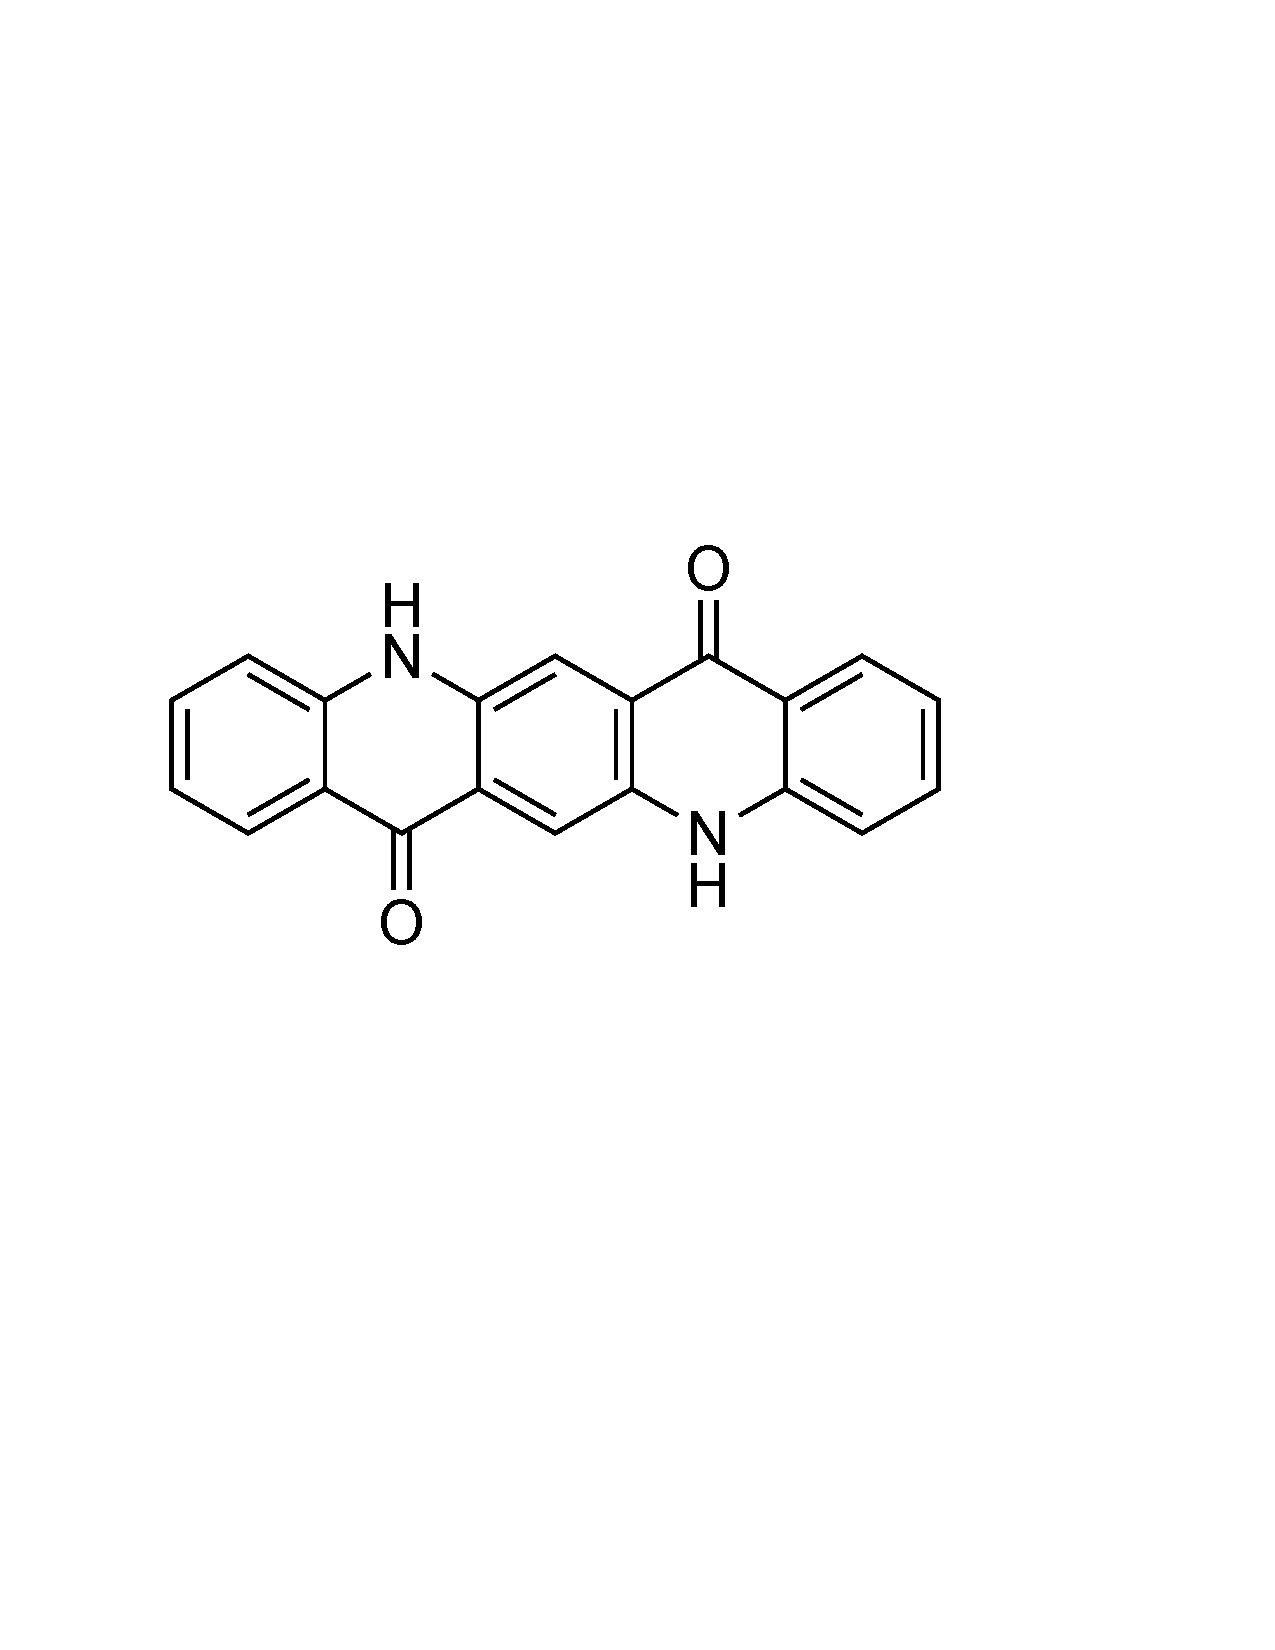
\includegraphics[width=\linewidth]{images/vertiefer/QA.pdf}
		\caption{Skeletal structure}
	\end{subfigure}
	\hfill
	\begin{subfigure}[b]{0.48\linewidth}
		\centering
		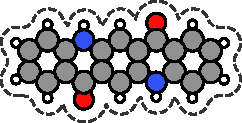
\includegraphics[width=\linewidth]{images/qa.pdf}
		\caption{Space-filling model}
	\end{subfigure}
\end{figure}

\end{frame}

%%%%%%%%%%%%%%
\begin{frame}
\frametitle{$\alpha$-phase of QA on Ag(100)\autocite{Humberg2025}}

\begin{figure}
    \centering
    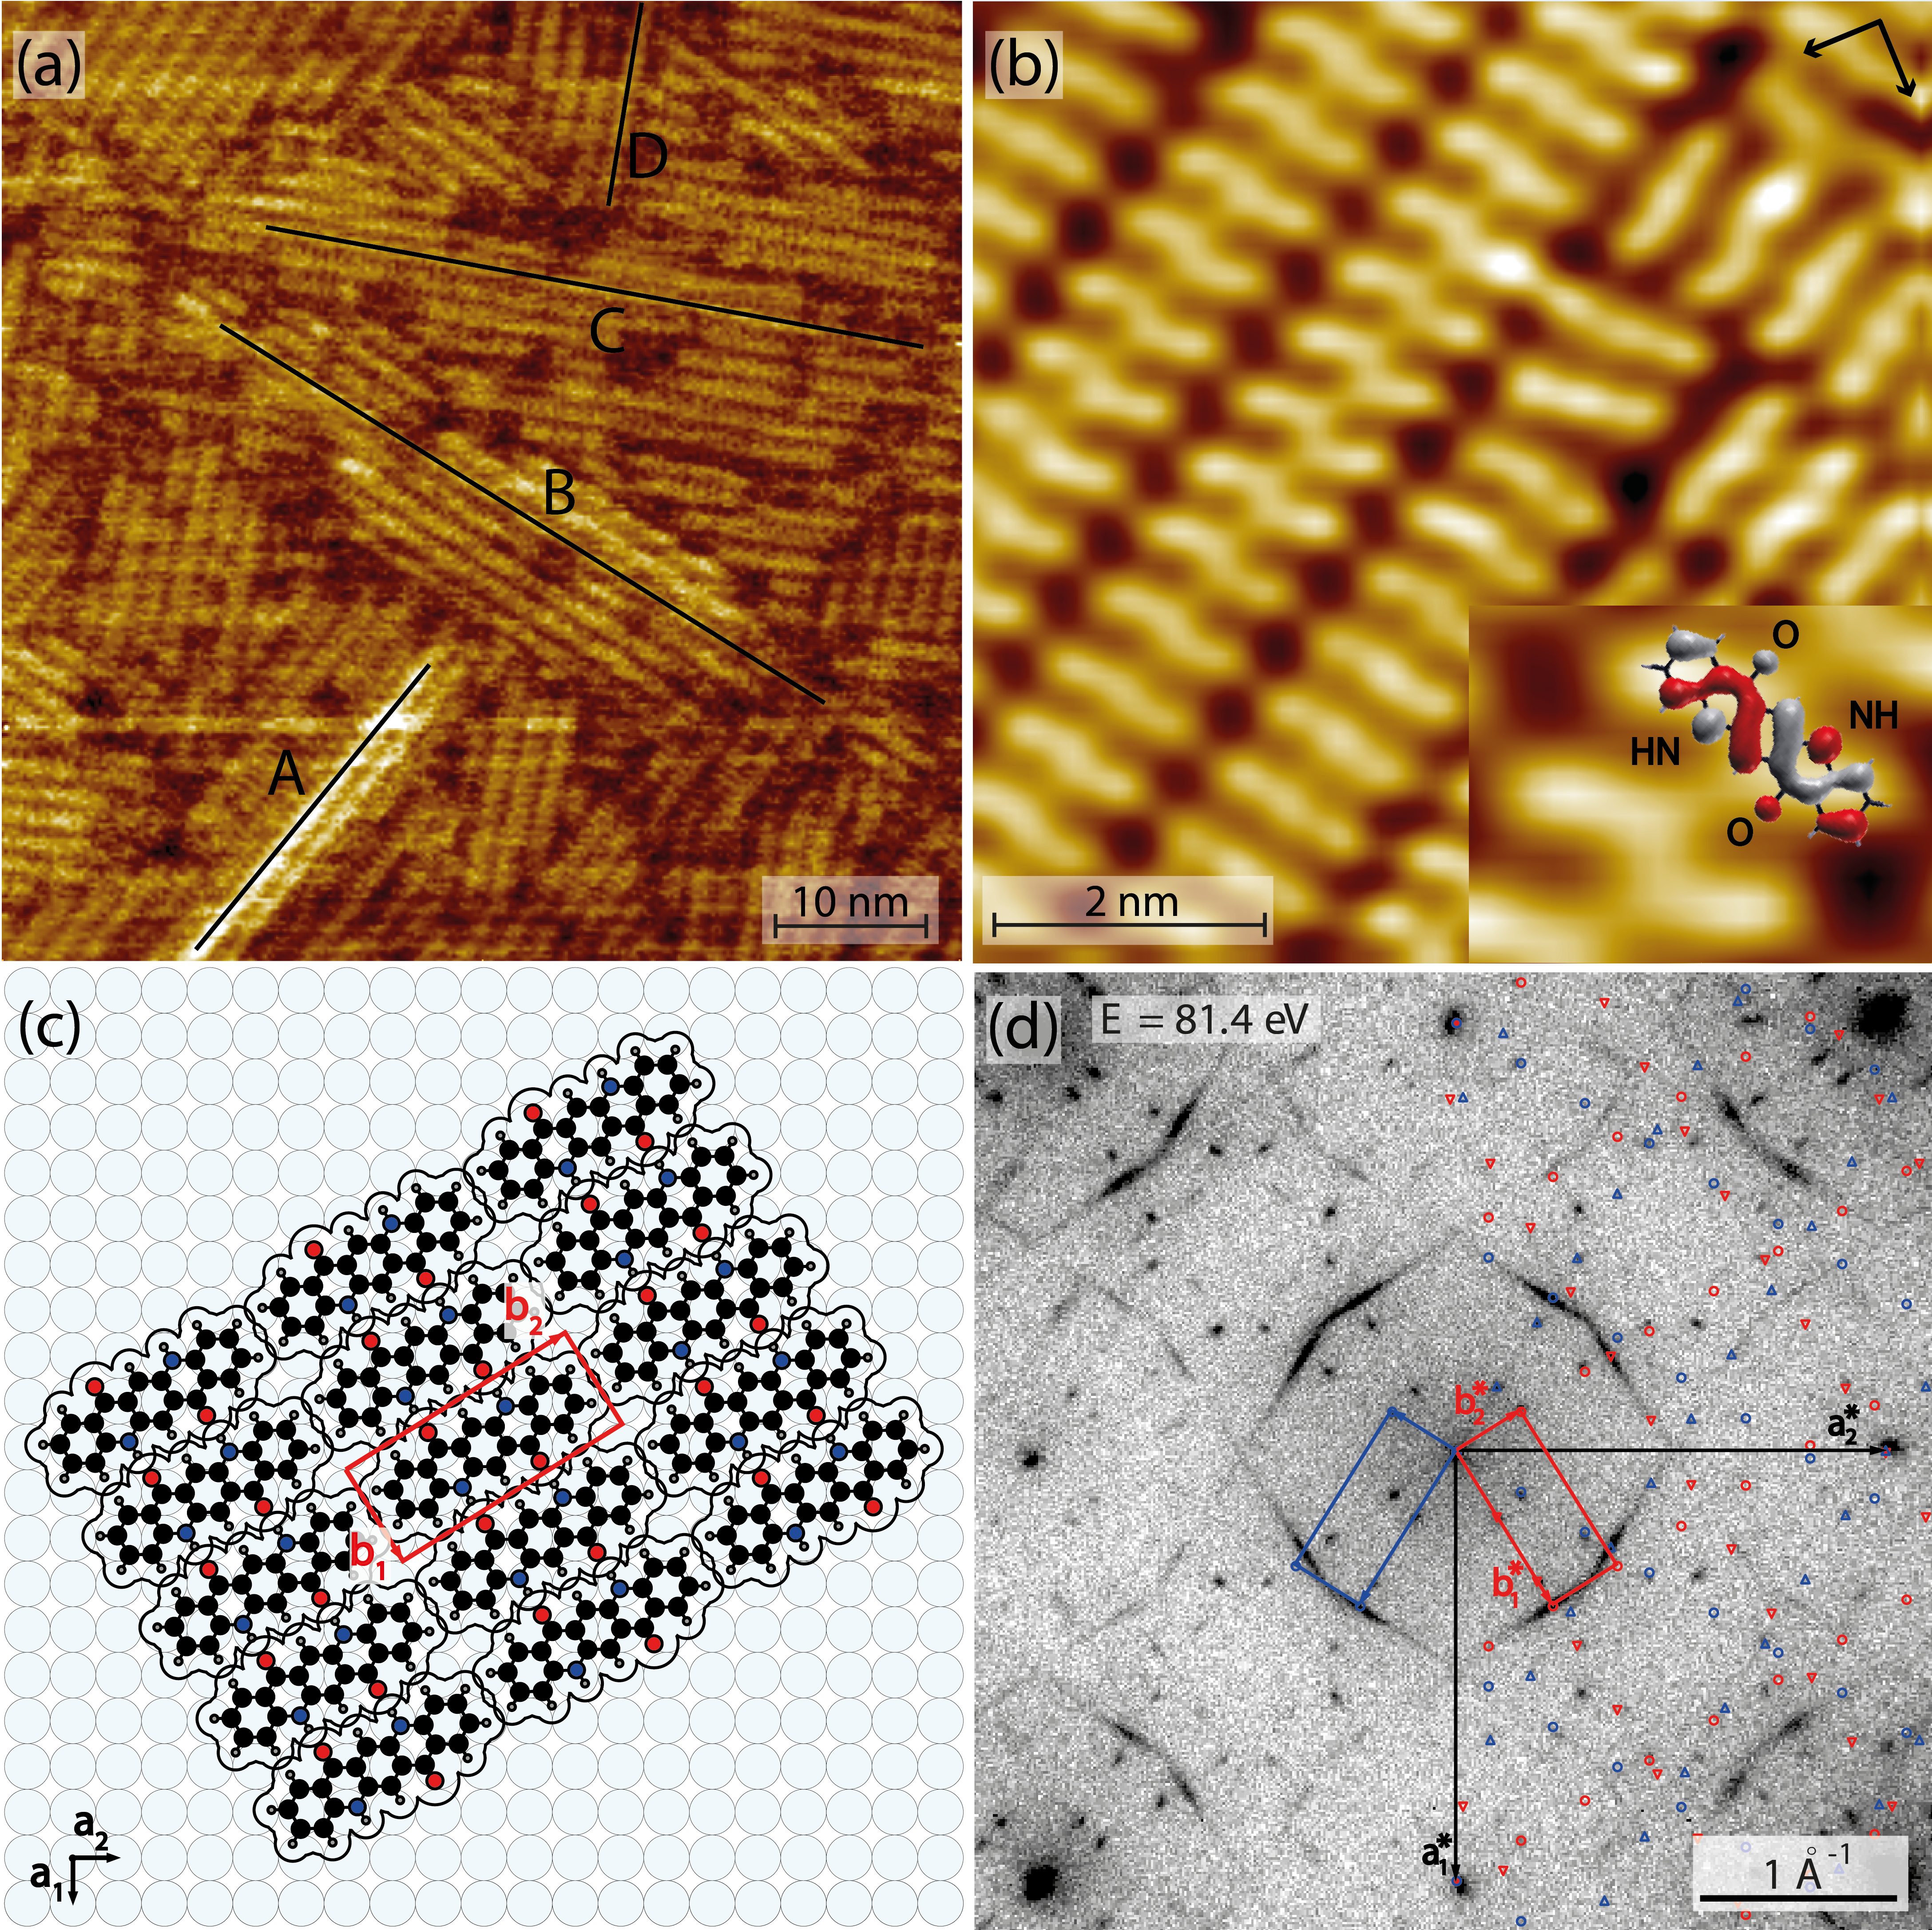
\includegraphics[width=0.6\textwidth]{images/vertiefer/literature_alpha.png}
    \caption{Literature overview of the $\alpha$-phase of QA on Ag(100).}
    \label{fig:literature_alpha}
\end{figure}

\end{frame}

%%%%%%%%%%%%%%
\begin{frame}
\frametitle{$\beta$-phase of QA on Ag(100)\autocite{Humberg2025}}

\begin{figure}
    \centering
    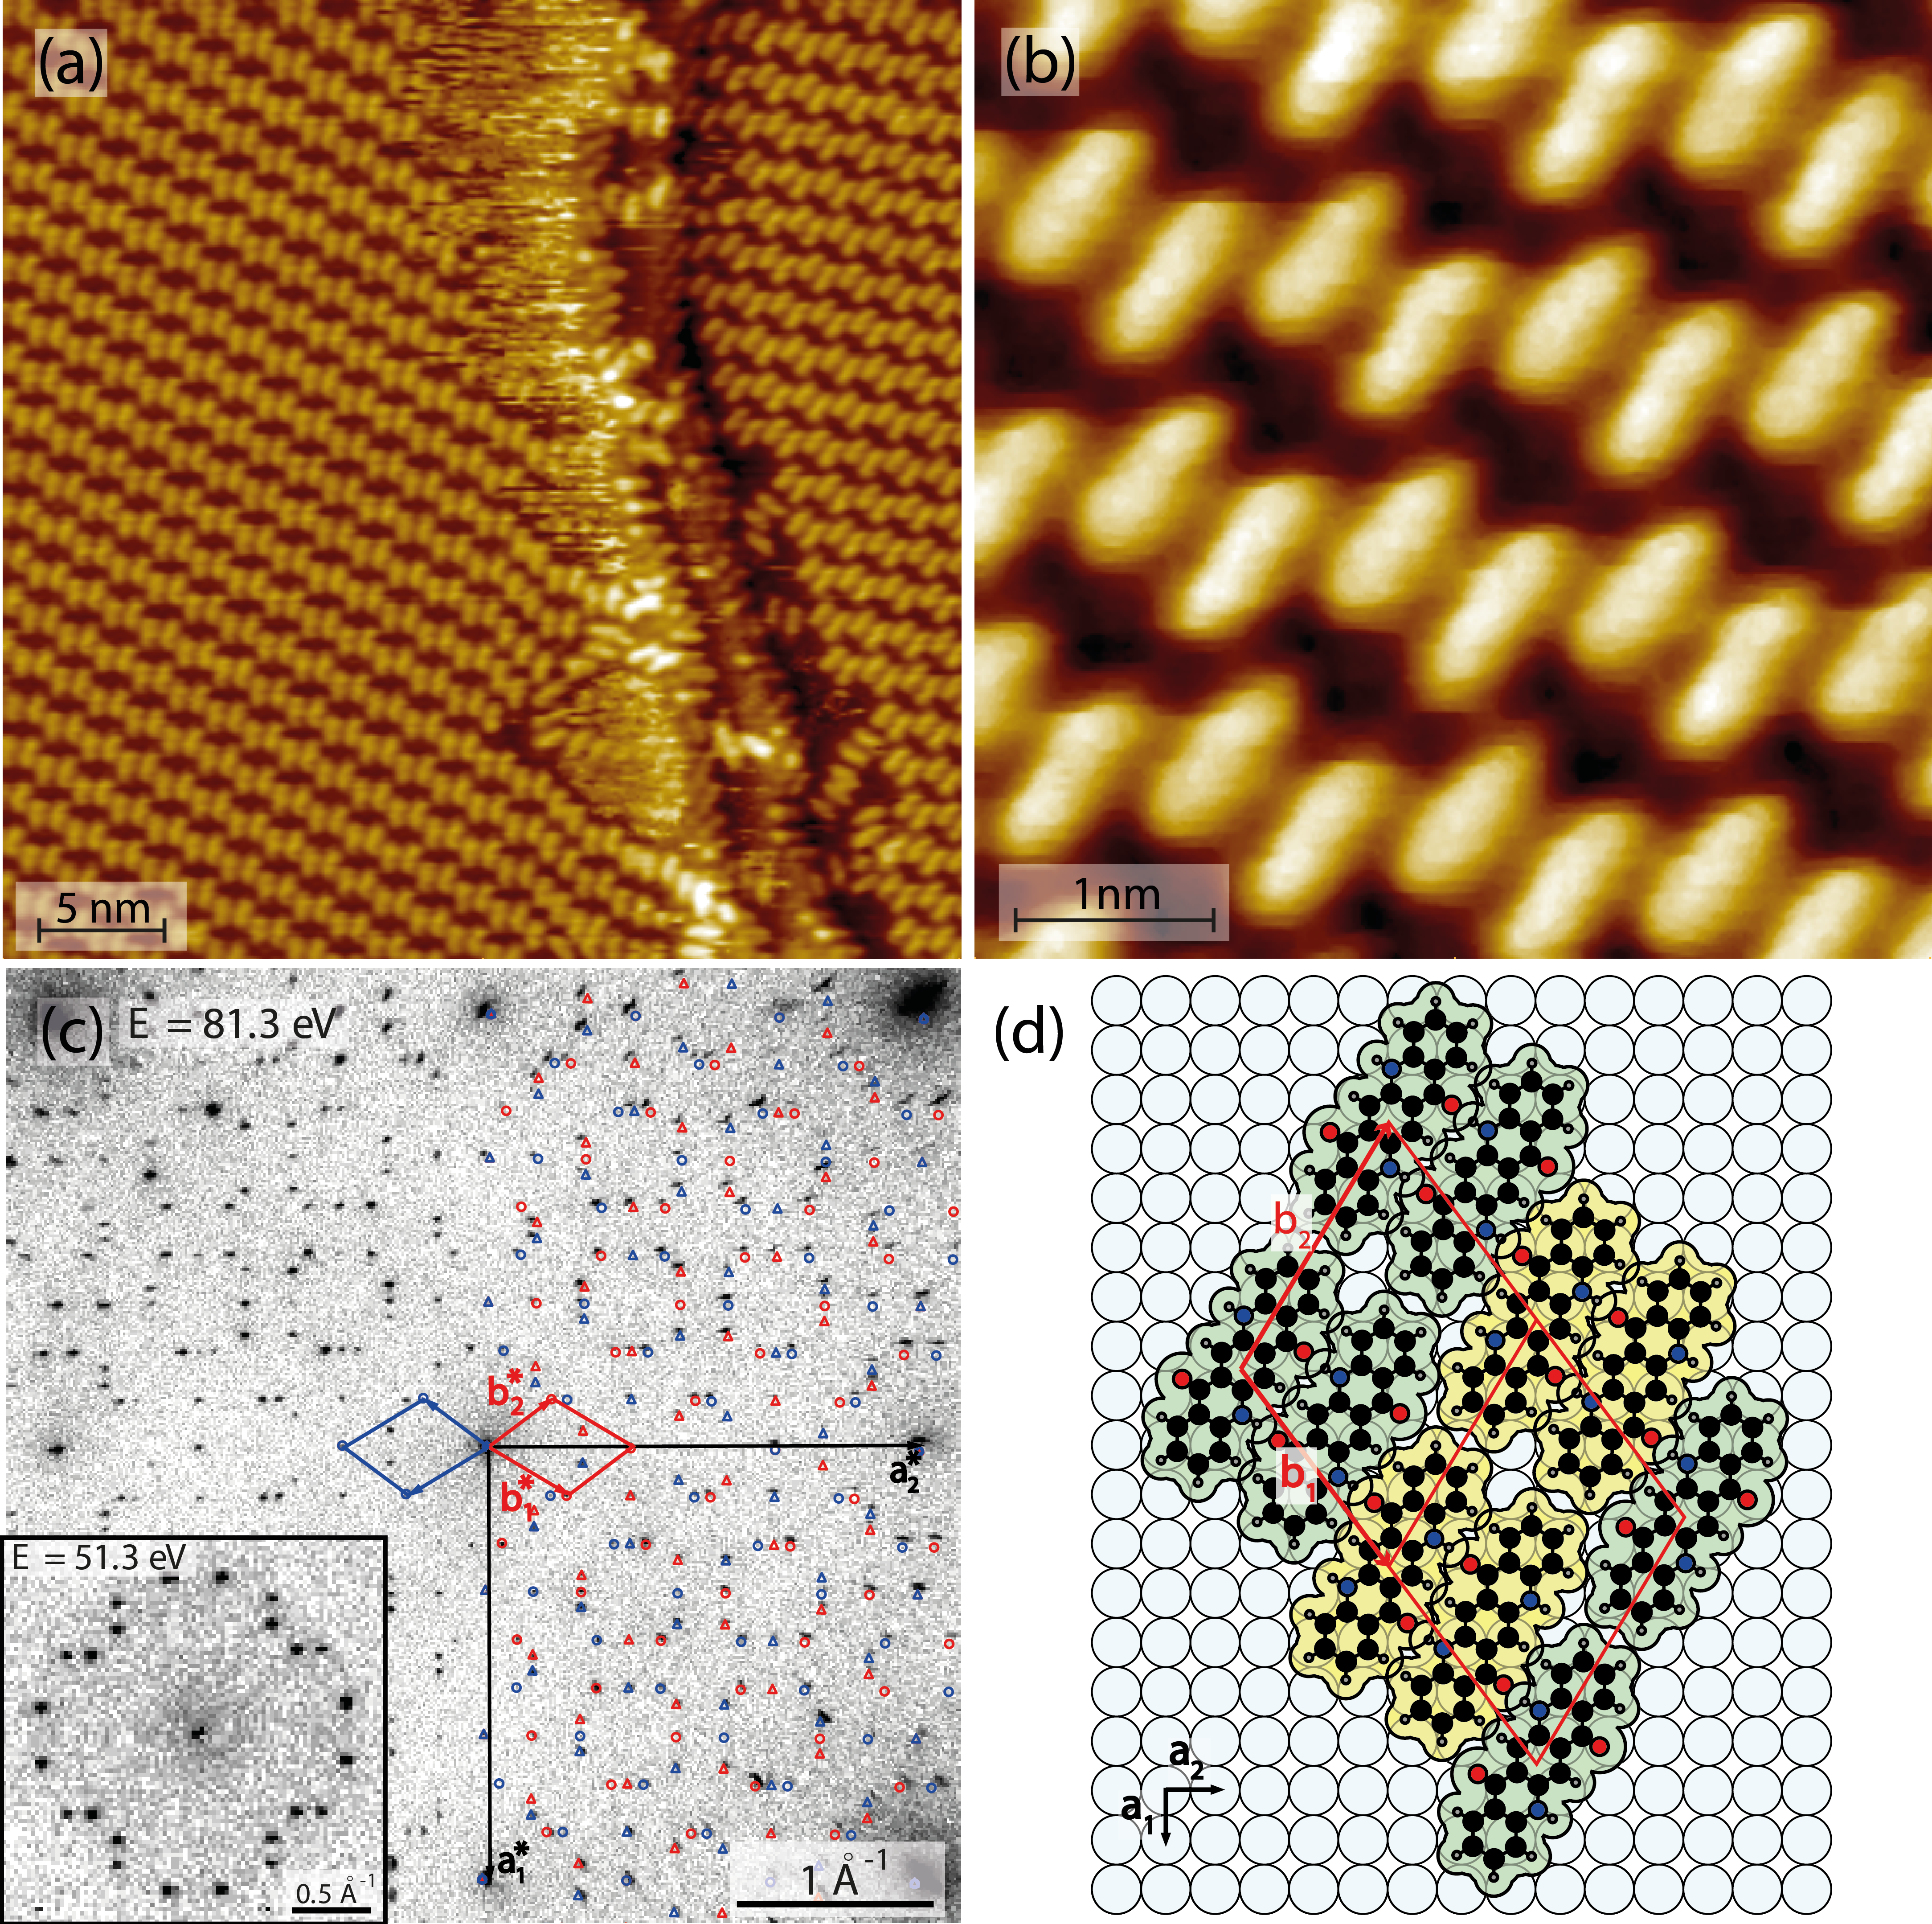
\includegraphics[width=0.6\textwidth]{images/vertiefer/literature_beta.png}
    \caption{Literature overview of the $\beta$-phase of QA on Ag(100).}
    \label{fig:literature_beta}
\end{figure}

\end{frame}

%%%%%%%%%%%%%%%%%%%%%%%%%%%%%%%%%%%%%%%%%%%%%%%%%%%%%%%%%%%%%%%%%%%
\section{Experimental/Theory}

\begin{frame}
\frametitle{XPS}

\begin{figure}
    \centering
    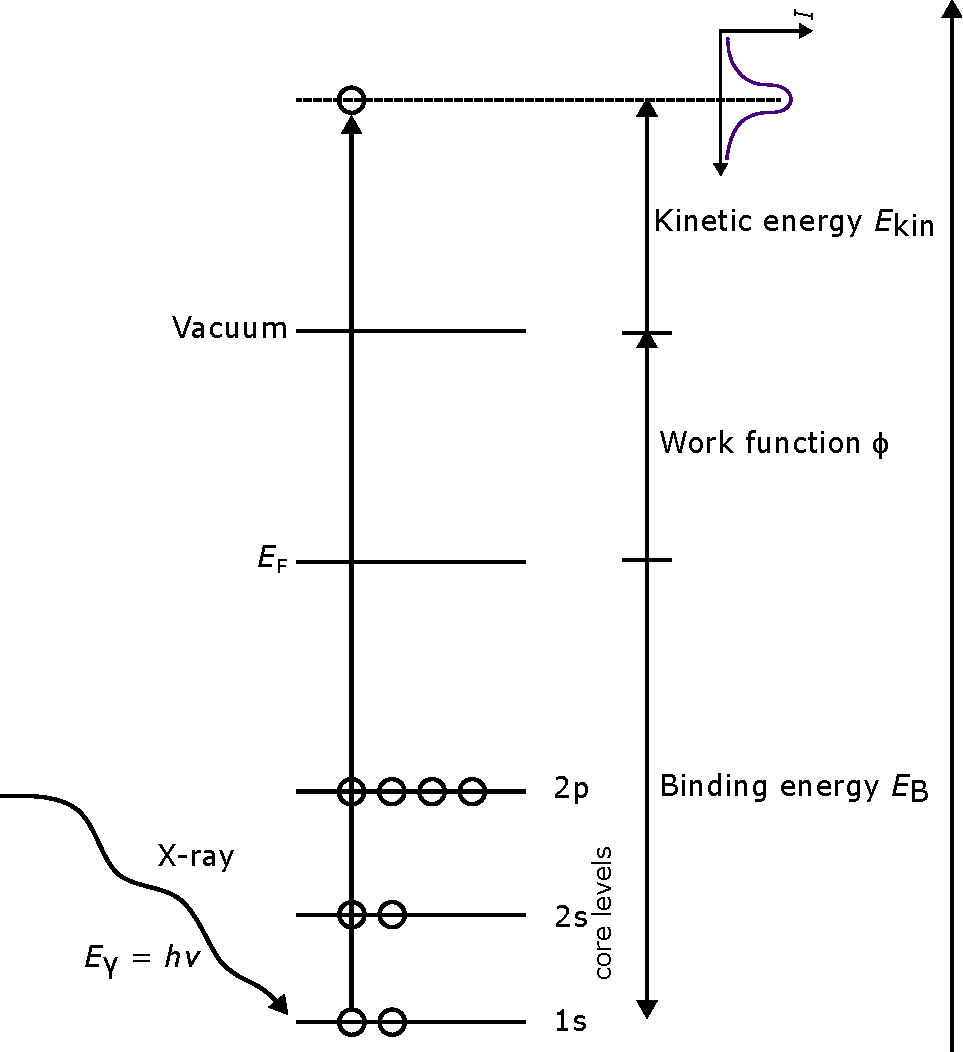
\includegraphics[width=0.55\textwidth]{images/vertiefer/XPS_schematic.pdf}
    \caption{Schematic illustration of the XPS process.}
    \label{fig:XPS}
\end{figure}

\end{frame}

%%%%%%%%%%%%%%
\begin{frame}
\frametitle{NIXSW}

\begin{figure}
    \centering
    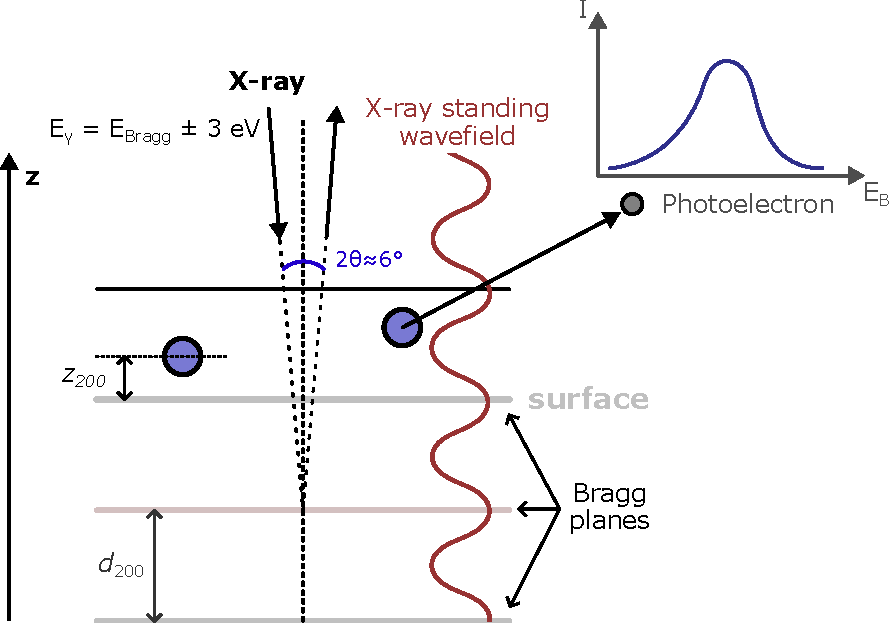
\includegraphics[width=0.8\textwidth]{images/NIXSW-theo.pdf}
    \caption{Schematic illustration of the NIXSW technique.}
    \label{fig:NIXSW}
\end{figure}

\end{frame}

%%%%%%%%%%%%%%
\begin{frame}
\frametitle{NIXSW}

\begin{figure}
  \centering
  \begin{subfigure}{0.45\textwidth}
    \centering
    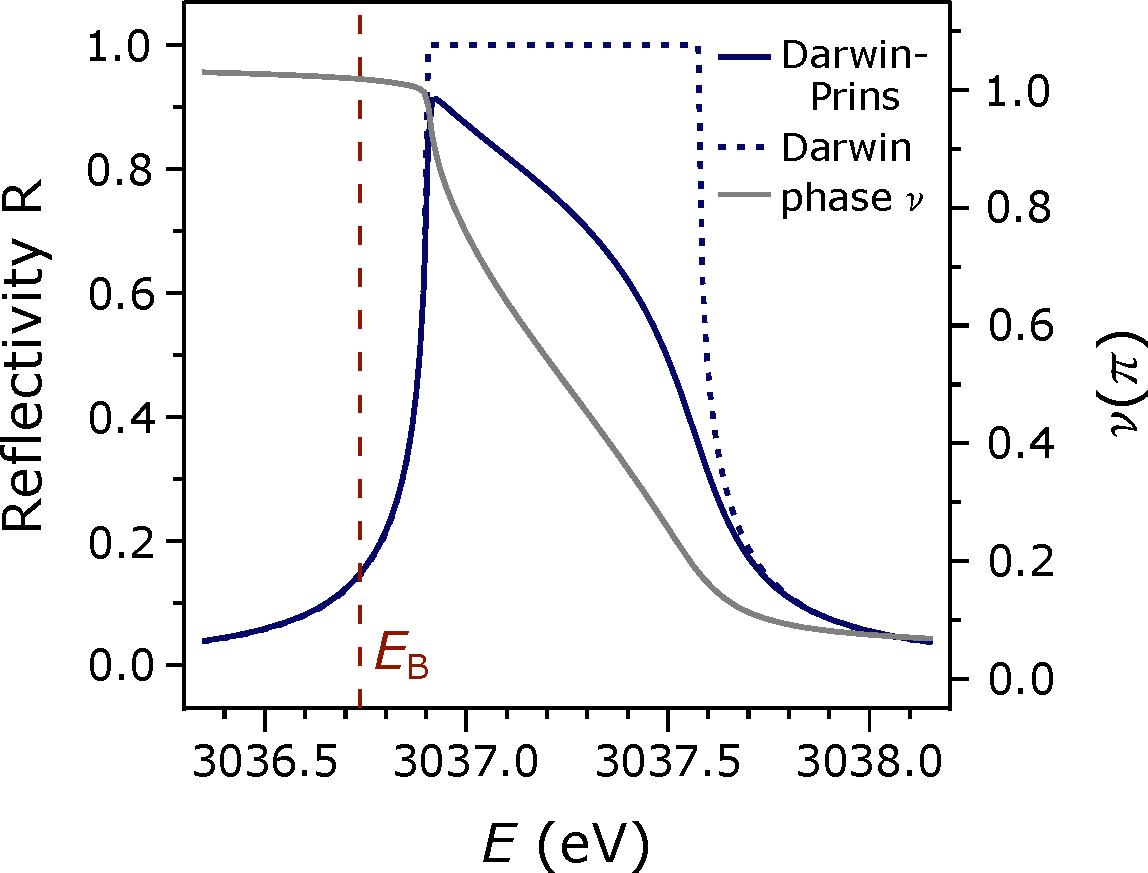
\includegraphics[width=\textwidth]{images/Reflectivity.pdf}
    \caption{Reflectivity}
  \end{subfigure}
  \hfill
  \begin{subfigure}{0.45\textwidth}
    \centering
    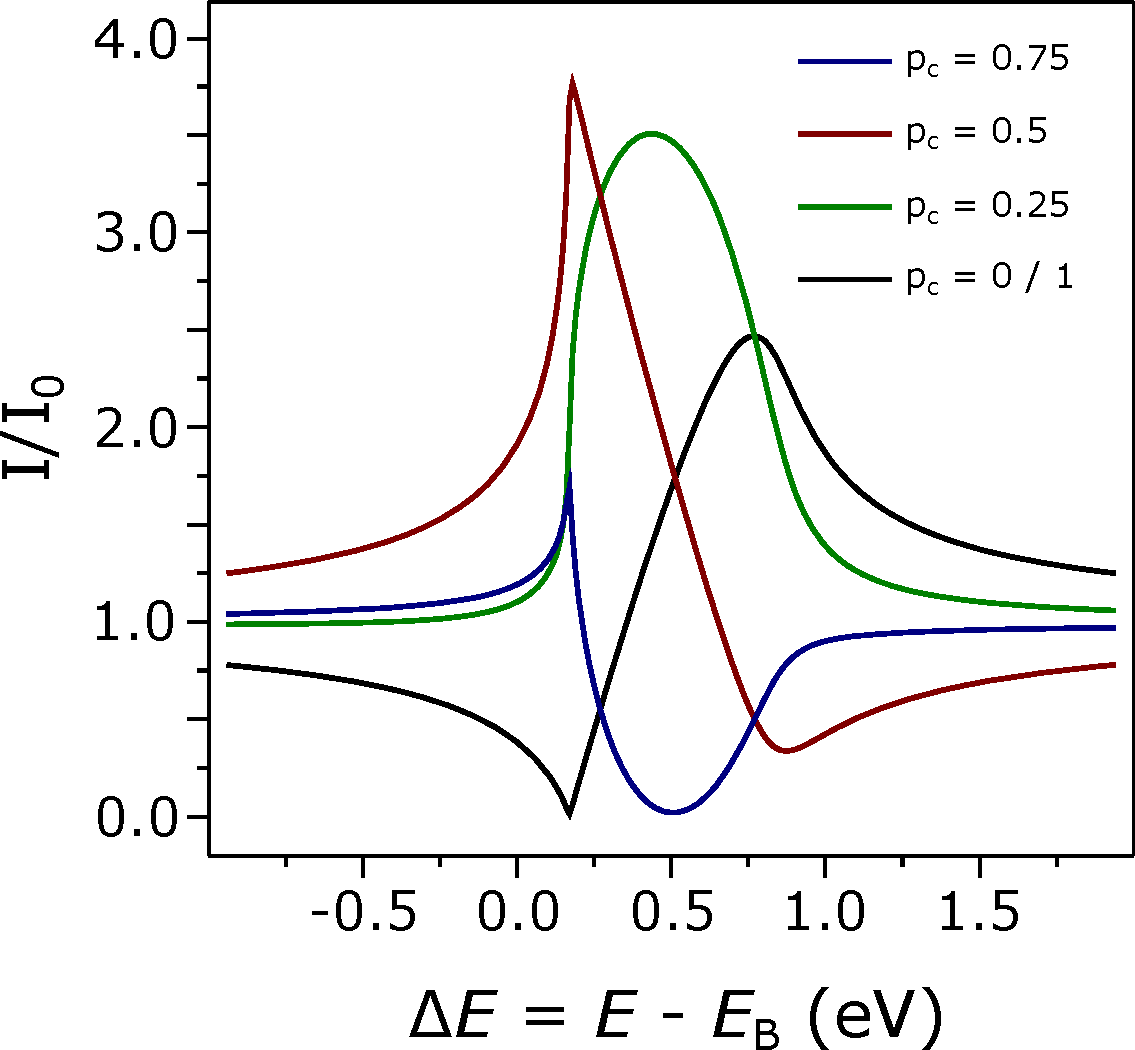
\includegraphics[width=\textwidth]{images/Yield.pdf}
    \caption{Yield}
  \end{subfigure}
\end{figure}

\begin{equation}
	\frac{I}{I_0} = 1 + S_\mathrm{R} R(E_\mathrm{\gamma}) + 2 |S_\mathrm{I}| \sqrt{R(E_\mathrm{\gamma})} \underbrace{f_\mathrm{c}} \cos(\nu(E_\mathrm{\gamma}) - 2\pi \underbrace{{p_\mathrm{c}}} + \psi)
\end{equation}

\end{frame}

%%%%%%%%%%%%%%%%%%%%%%%%%%%%%%%%%%%%%%%%%%%%%%%%%%%%%%%%%%%%%%%%%%%
\section{XPS of QA on Ag(100)}

\begin{frame}
\frametitle{XPS: C1s}

\begin{figure}
    \centering
    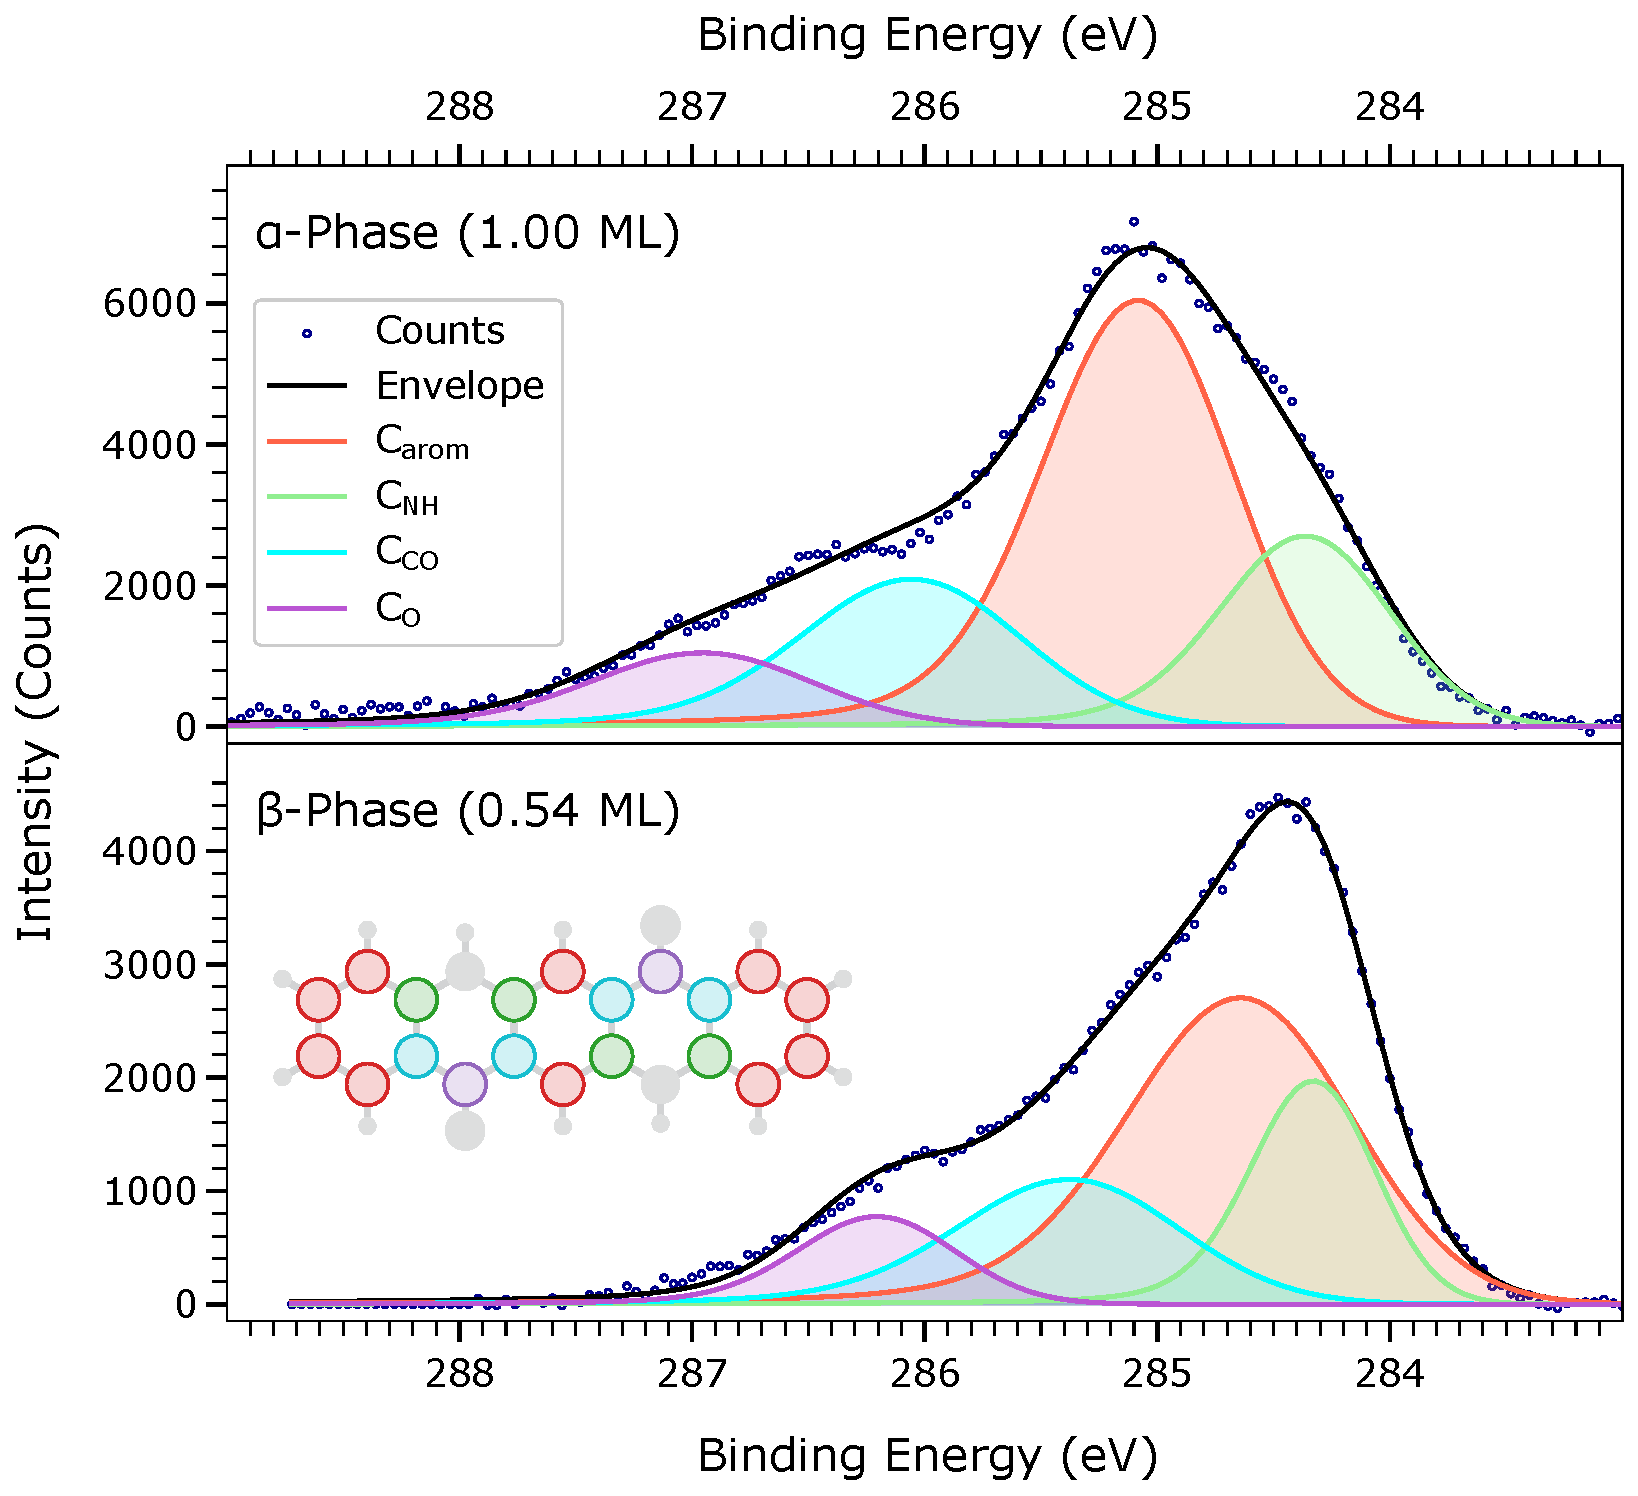
\includegraphics[width=0.7\textwidth]{images/XPS/C1s-Phases.pdf}
\end{figure}

\end{frame}

%%%%%%%%%%%%%%
\begin{frame}
\frametitle{XPS: N1s}

\begin{figure}
    \centering
    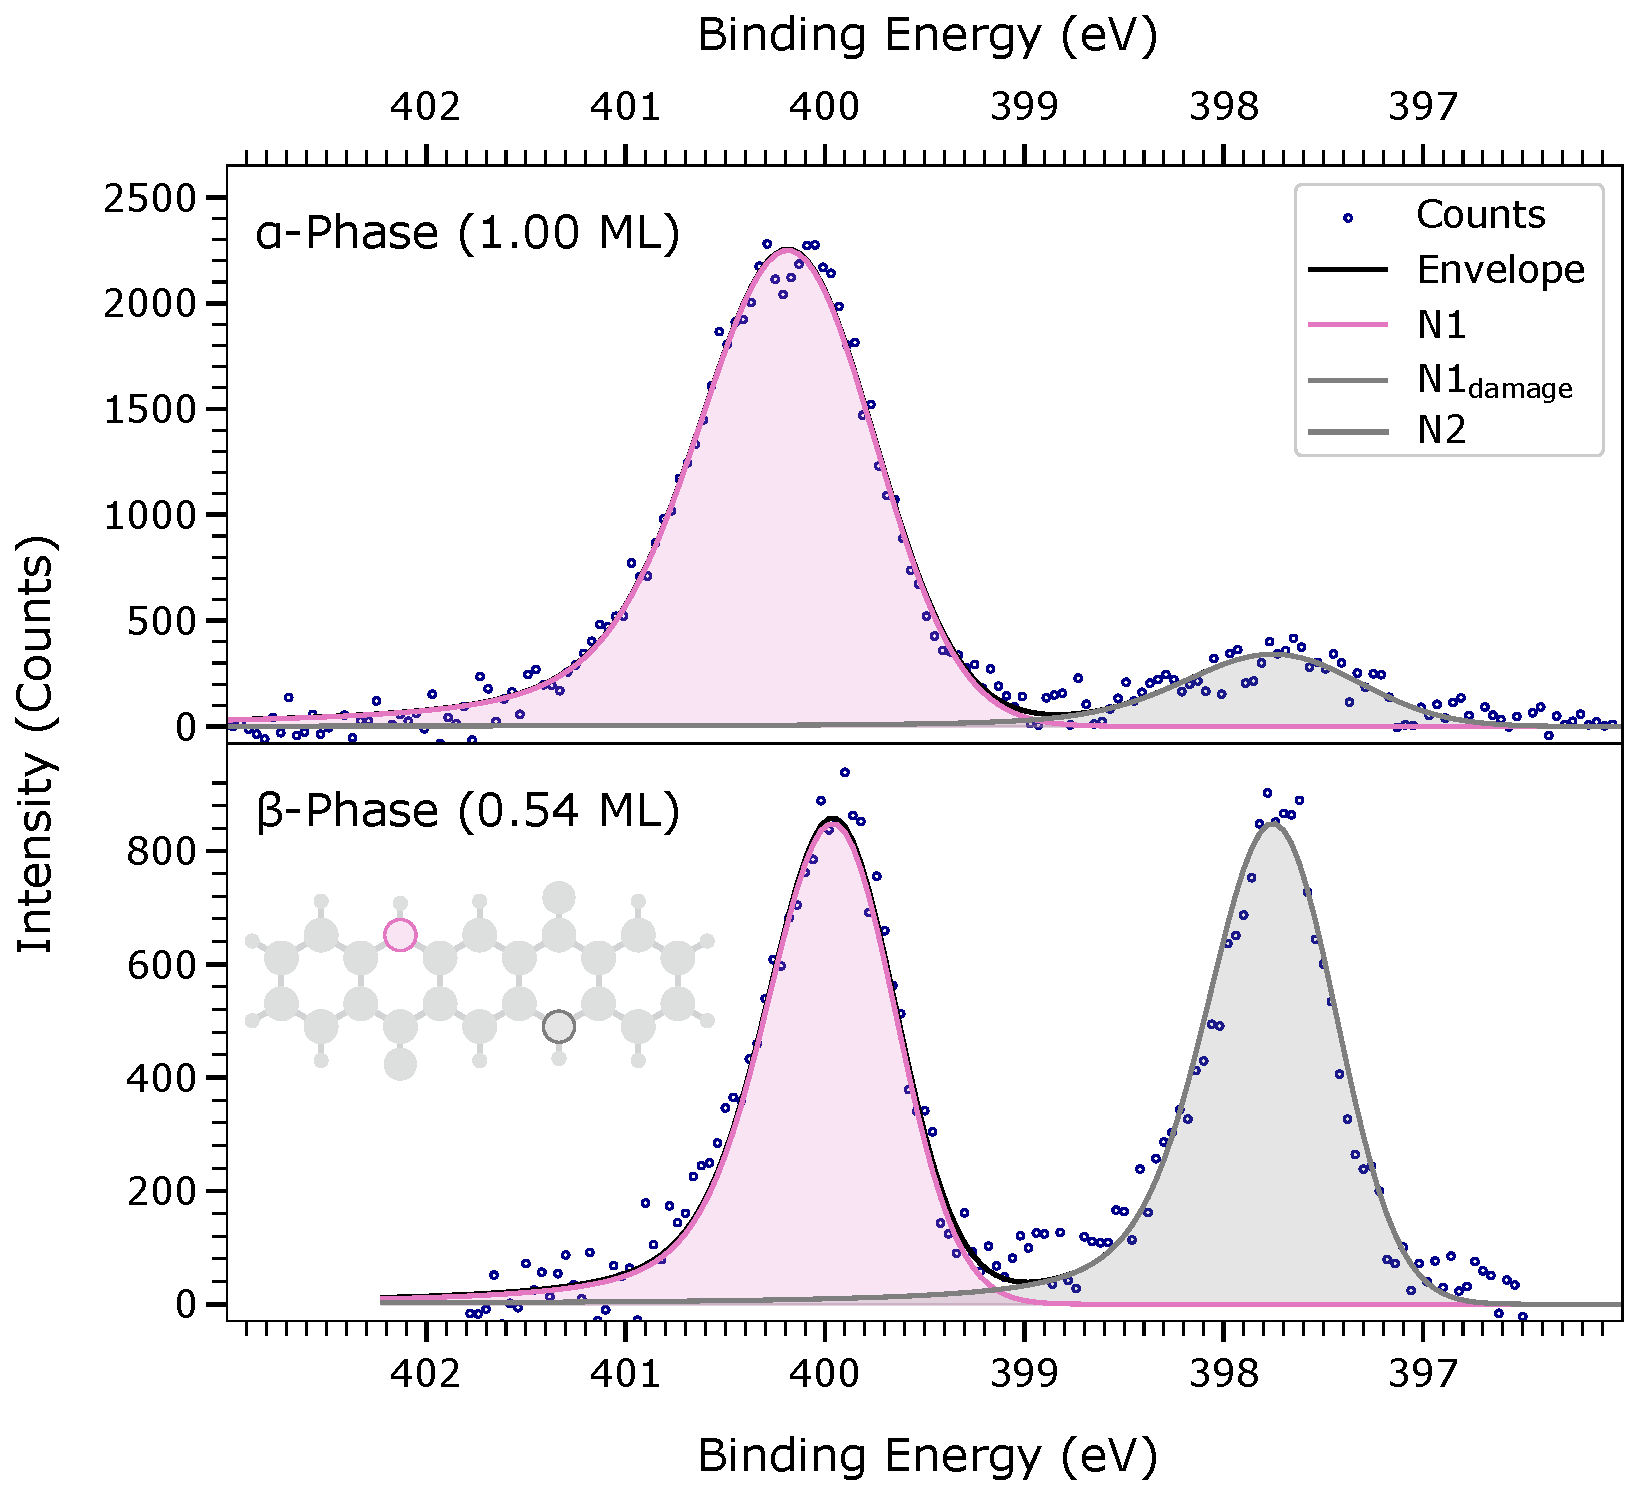
\includegraphics[width=0.7\textwidth]{images/XPS/N1s-Phases.pdf}
\end{figure}

\end{frame}

%%%%%%%%%%%%%%
\begin{frame}
\frametitle{XPS: O1s}

\begin{figure}
    \centering
    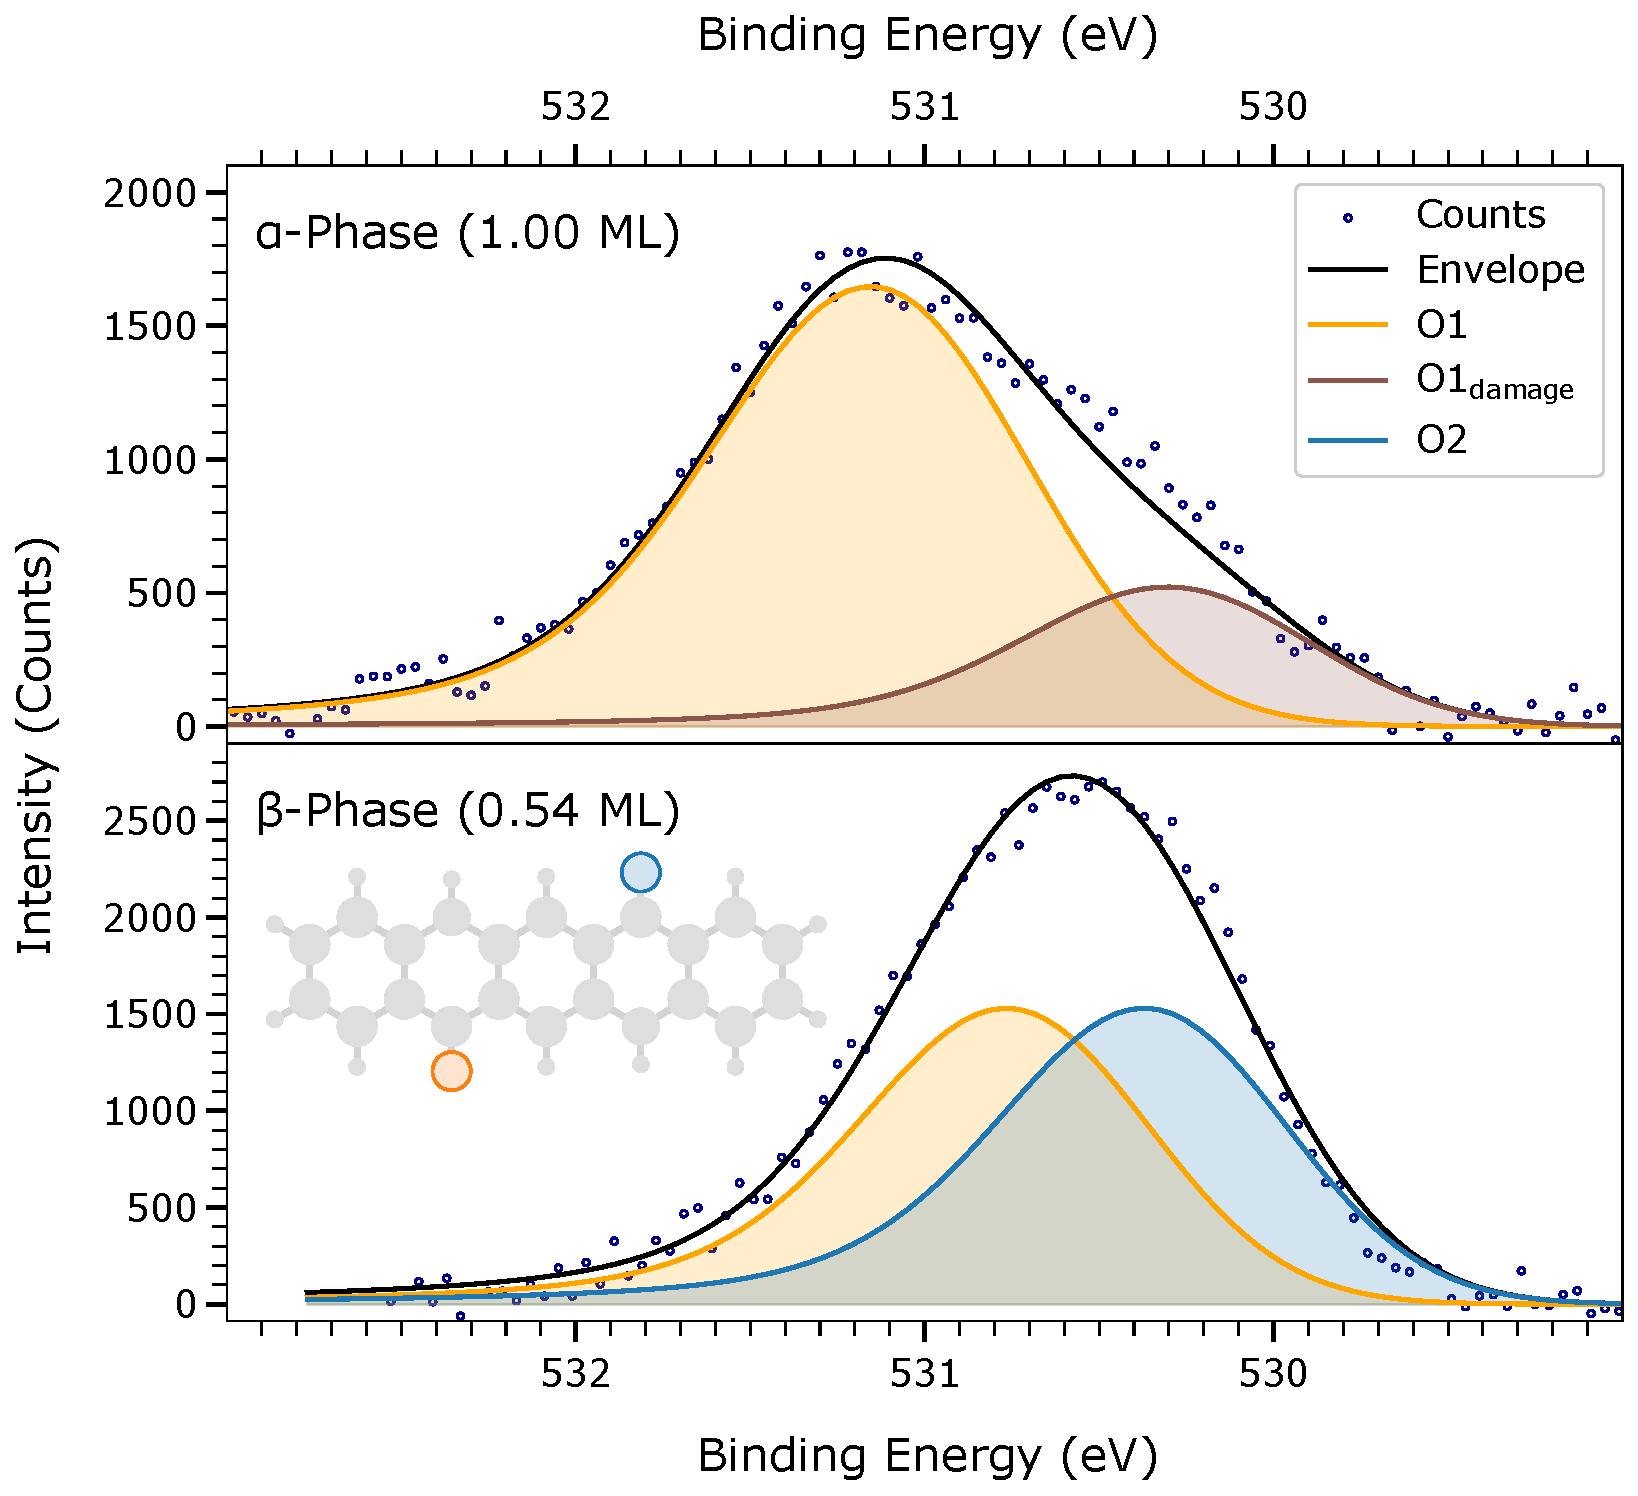
\includegraphics[width=0.7\textwidth]{images/XPS/O1s-Phases.pdf}
\end{figure}

\end{frame}

%%%%%%%%%%%%%%
\begin{frame}
\frametitle{XPS: C1s Phase transition}

\begin{figure}
    \centering
    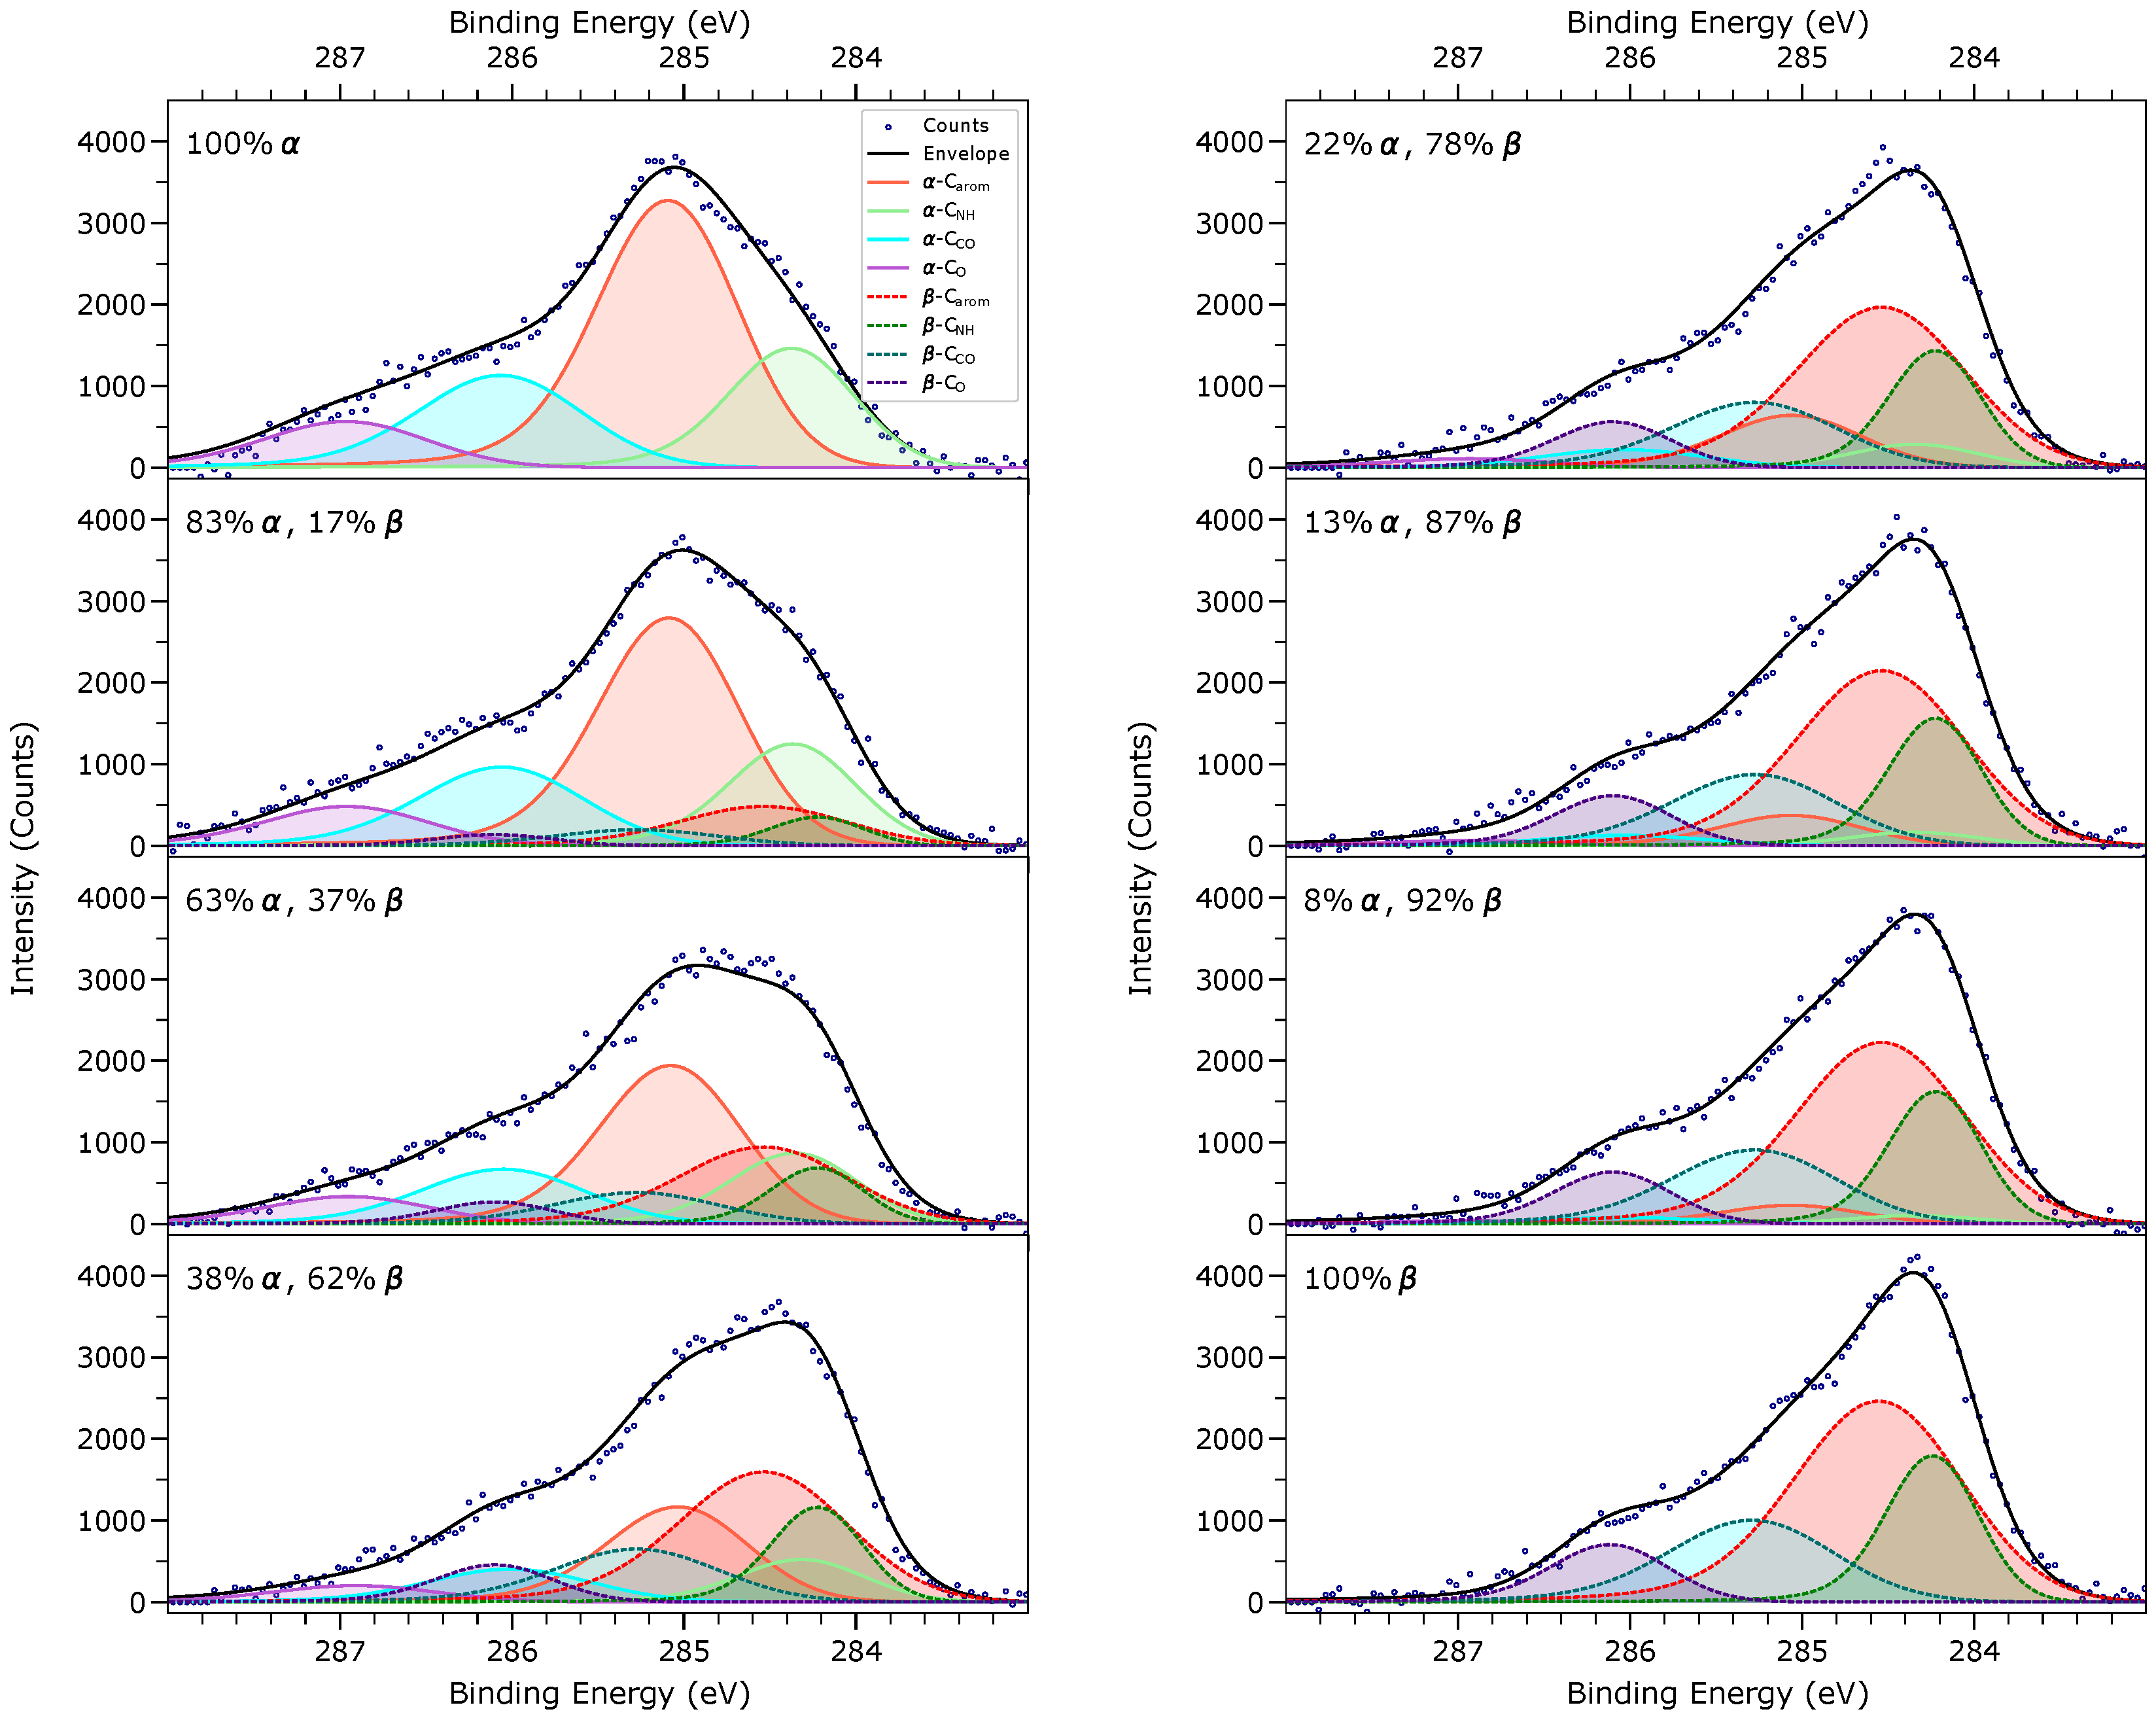
\includegraphics[width=0.75\textwidth]{images/XPS/C1s_Phase-Transition.pdf}
\end{figure}

\end{frame}


%%%%%%%%%%%%%%%%%%%%%%%%%%%%%%%%%%%%%%%%%%%%%%%%%%%%%%%%%%%%%%%%%%%
\section{NIXSW of QA on Ag(100)}

\begin{frame}
\frametitle{NIXSW: C1s}

\begin{figure}
	\centering
	\begin{subfigure}[b]{0.48\linewidth}
		\centering
		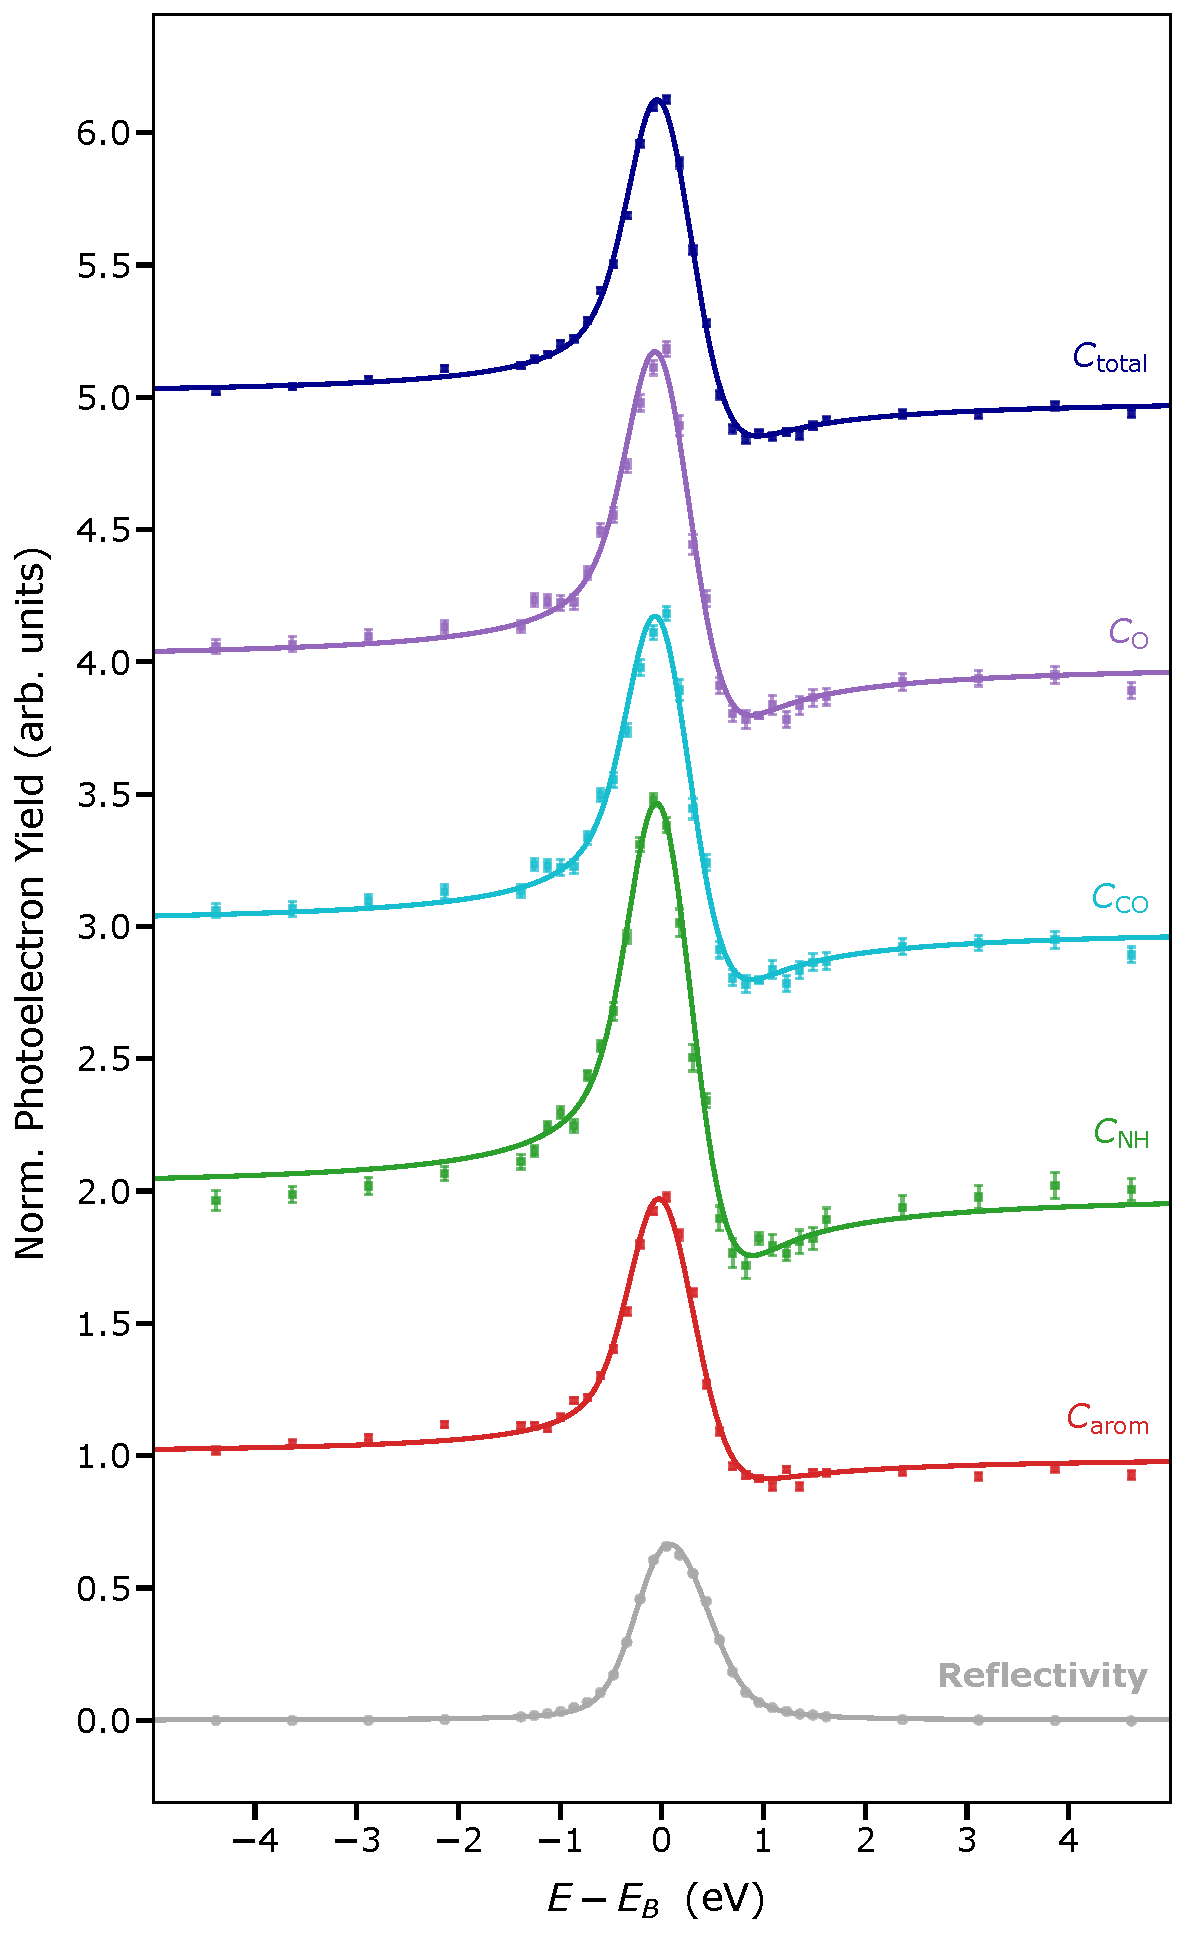
\includegraphics[width=0.75\linewidth]{images/NIXSW/NIXSW_C1s_Alpha.pdf}
		\caption{$\alpha$-phase}
	\end{subfigure}
	\hfill
	\begin{subfigure}[b]{0.48\linewidth}
		\centering
		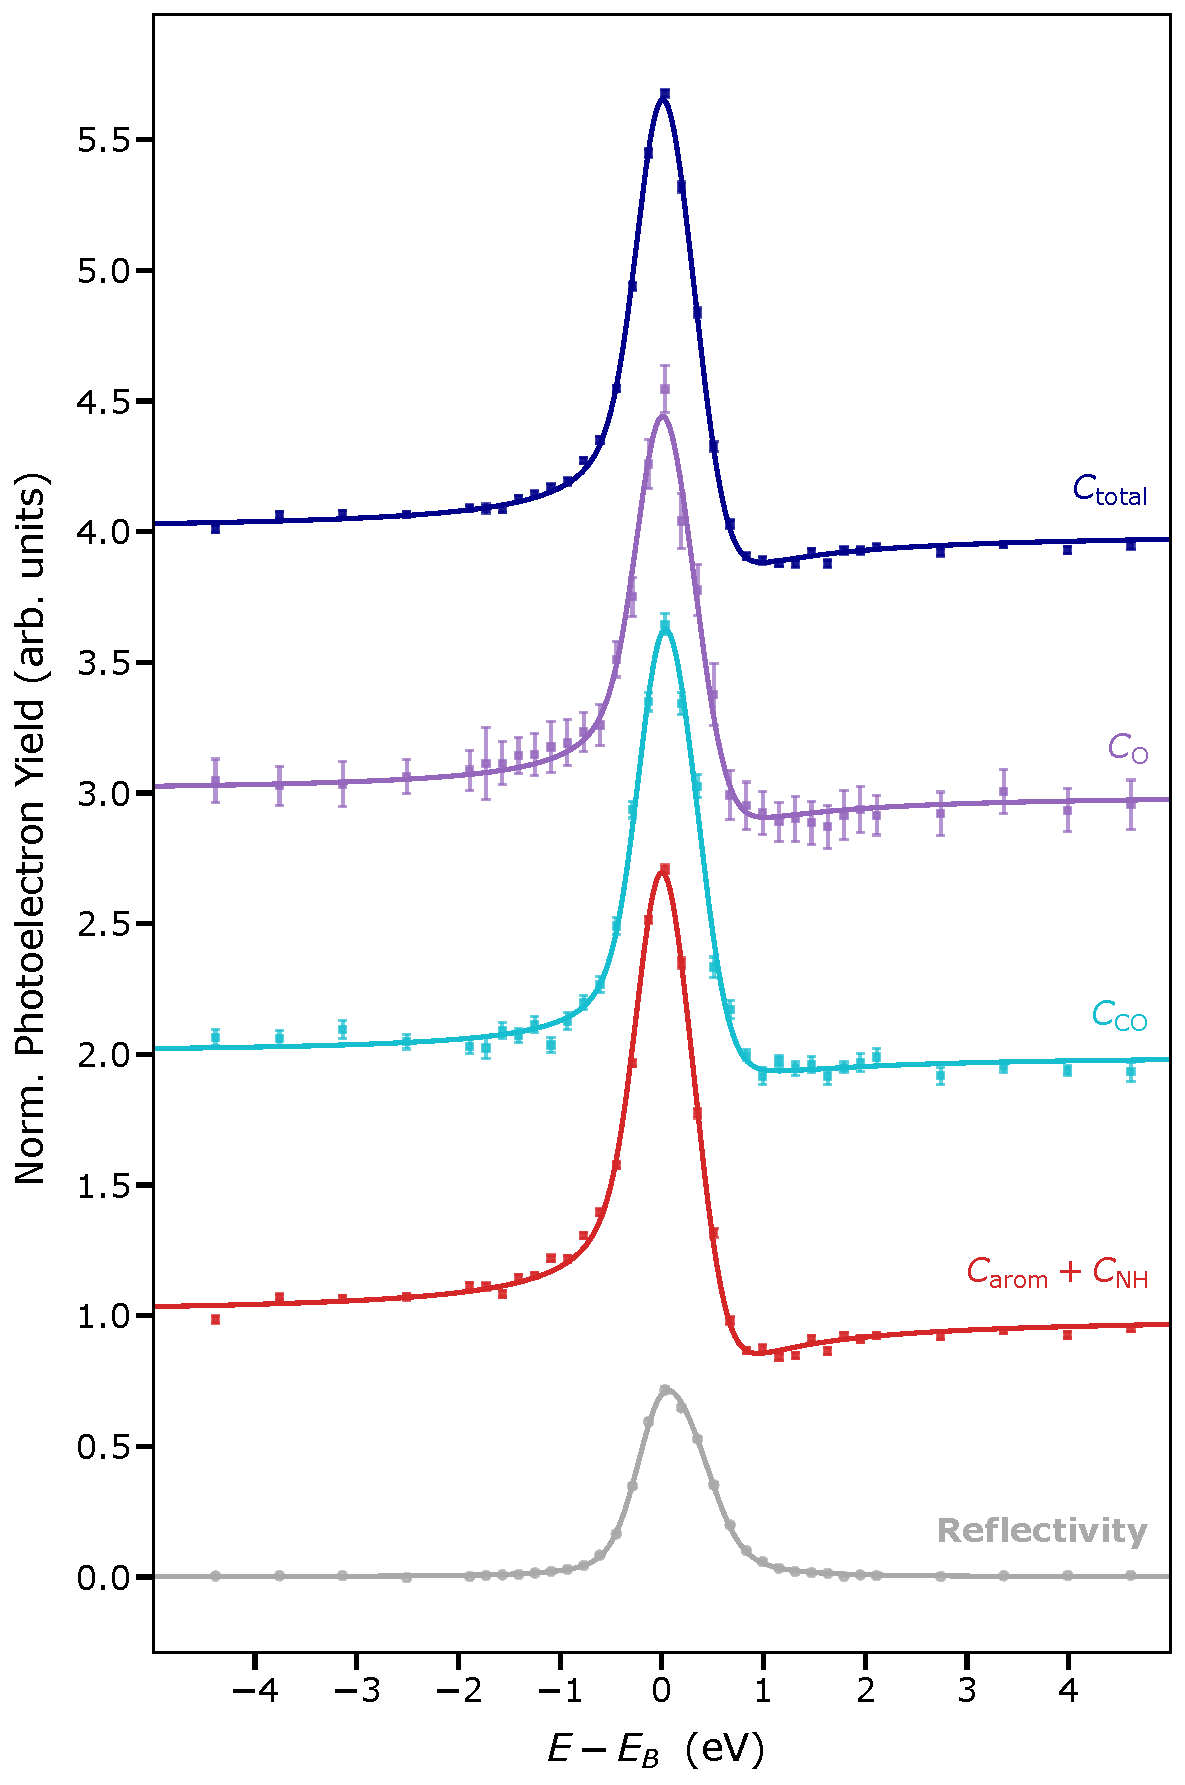
\includegraphics[width=0.75\linewidth]{images/NIXSW/NIXSW_C1s_Beta.pdf}
		\caption{$\beta$-phase}
	\end{subfigure}
\end{figure}

\end{frame}

%%%%%%%%%%%%%%
\begin{frame}
\frametitle{NIXSW: N1s}

\begin{figure}
	\centering
	\begin{subfigure}[b]{0.48\linewidth}
		\centering
		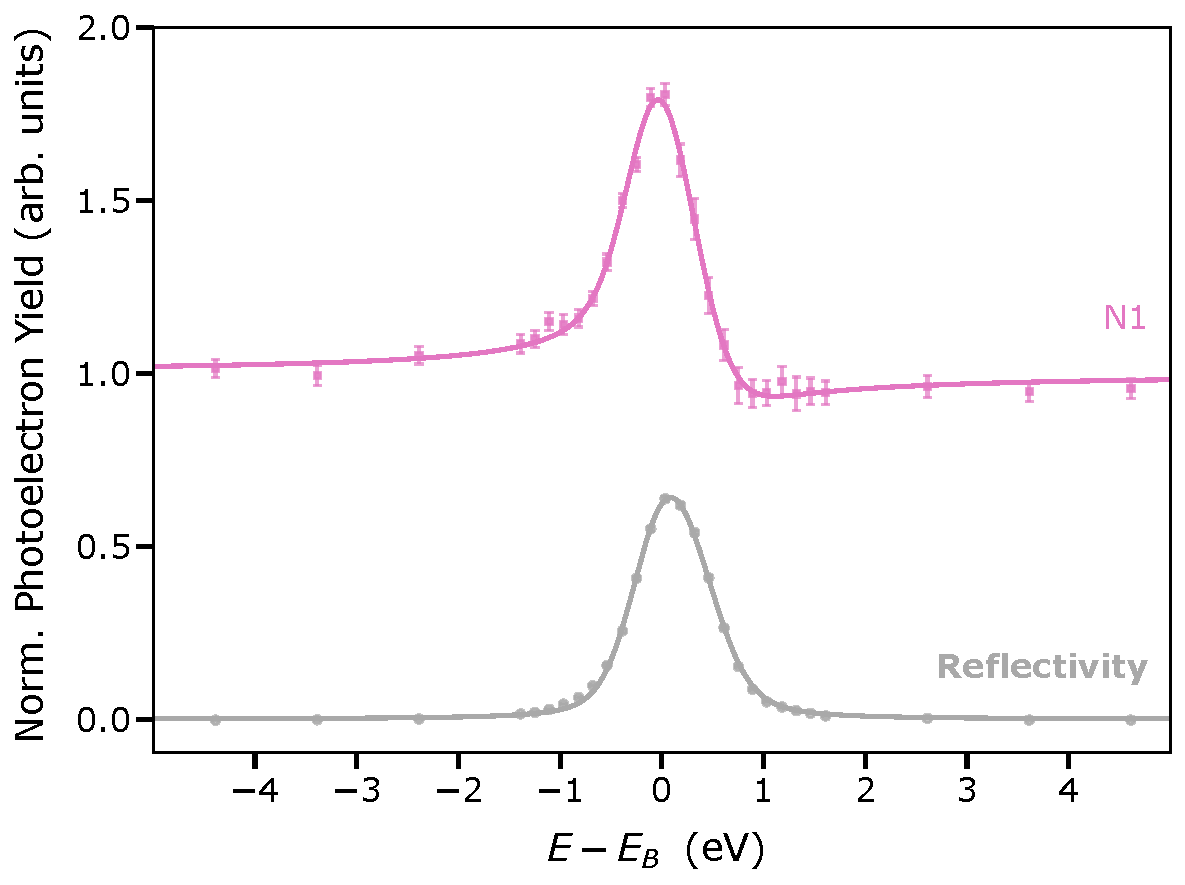
\includegraphics[width=\linewidth]{images/NIXSW/NIXSW_N1s_Alpha.pdf}
		\caption{$\alpha$-phase}
	\end{subfigure}
	\hfill
	\begin{subfigure}[b]{0.48\linewidth}
		\centering
		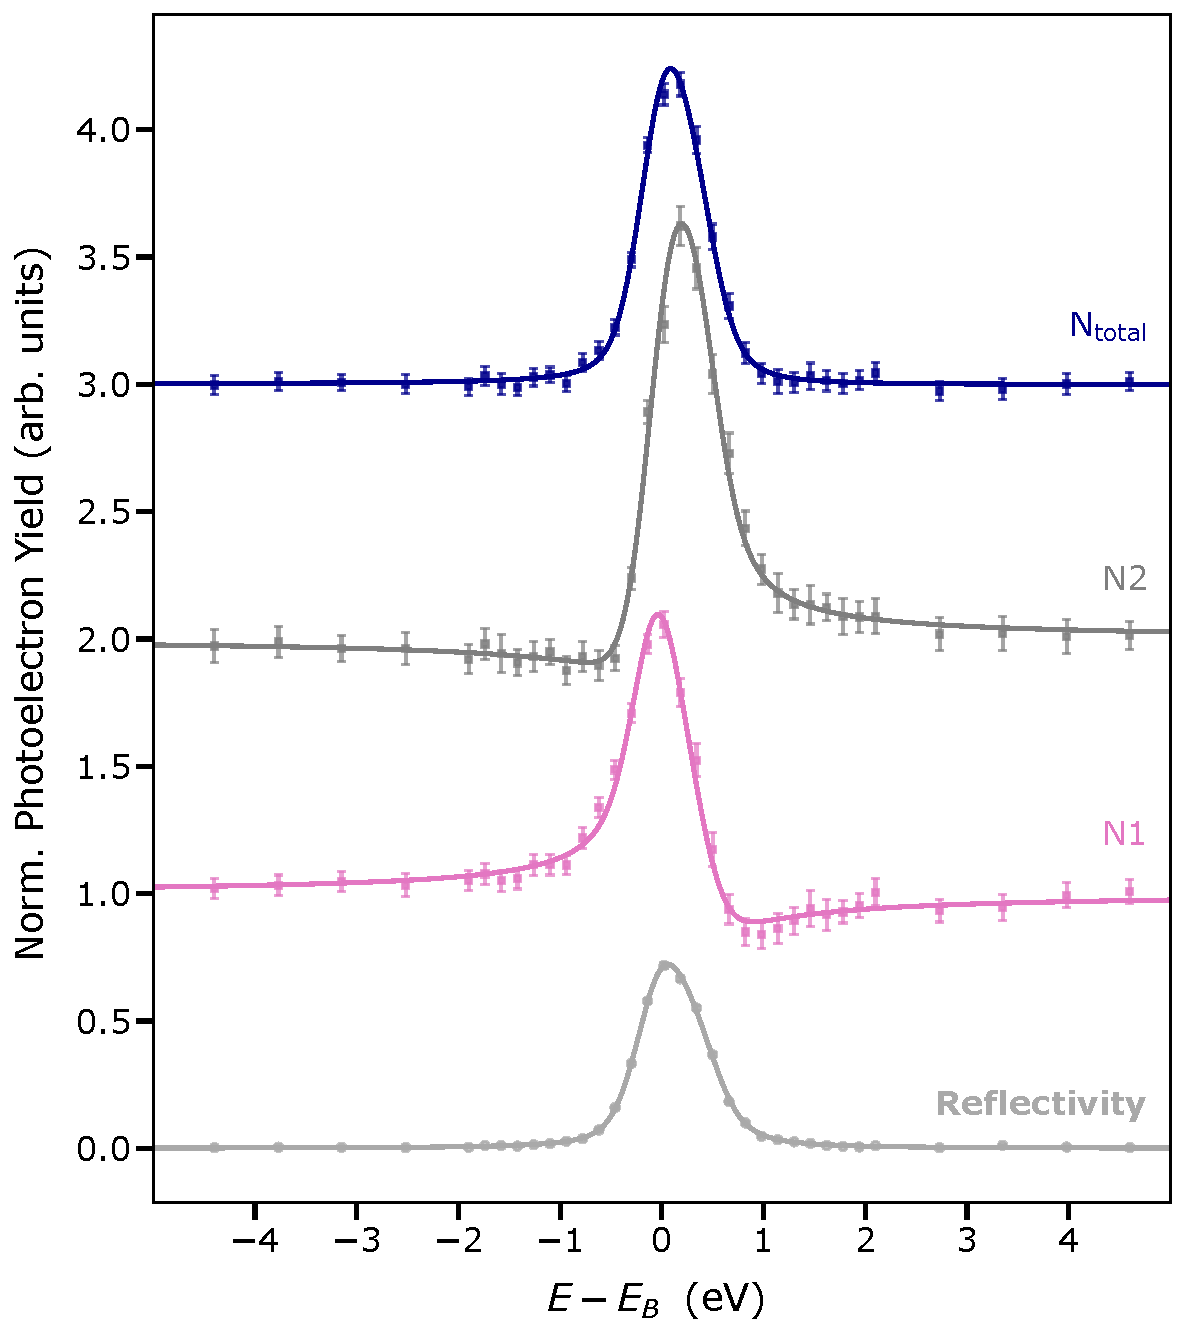
\includegraphics[width=\linewidth]{images/NIXSW/NIXSW_N1s_Beta.pdf}
		\caption{$\beta$-phase}
	\end{subfigure}
\end{figure}

\end{frame}

%%%%%%%%%%%%%%
\begin{frame}
\frametitle{NIXSW: O1s}

\begin{figure}
	\centering
	\begin{subfigure}[b]{0.48\linewidth}
		\centering
		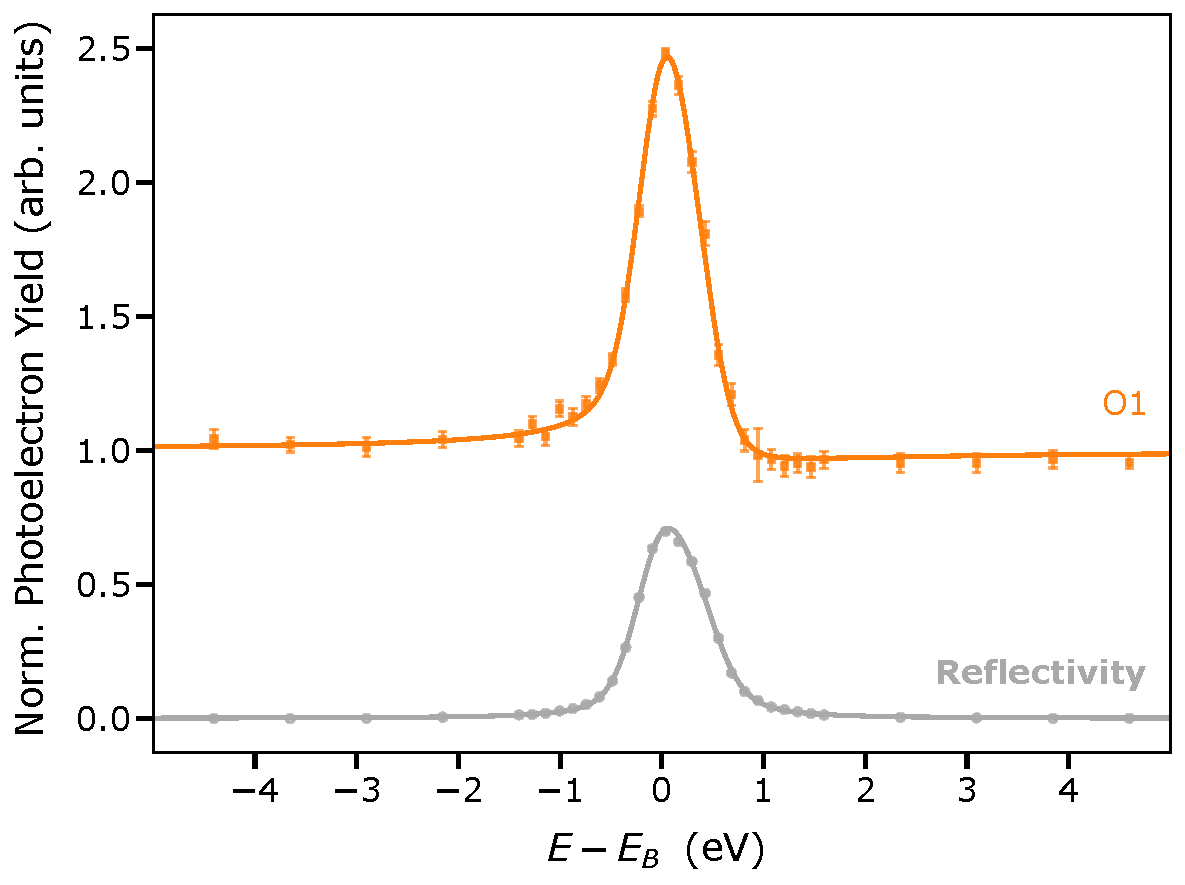
\includegraphics[width=0.75\linewidth]{images/NIXSW/NIXSW_O1s_Alpha.pdf}
		\caption{$\alpha$-phase}
	\end{subfigure}
	\hfill
	\begin{subfigure}[b]{0.48\linewidth}
		\centering
		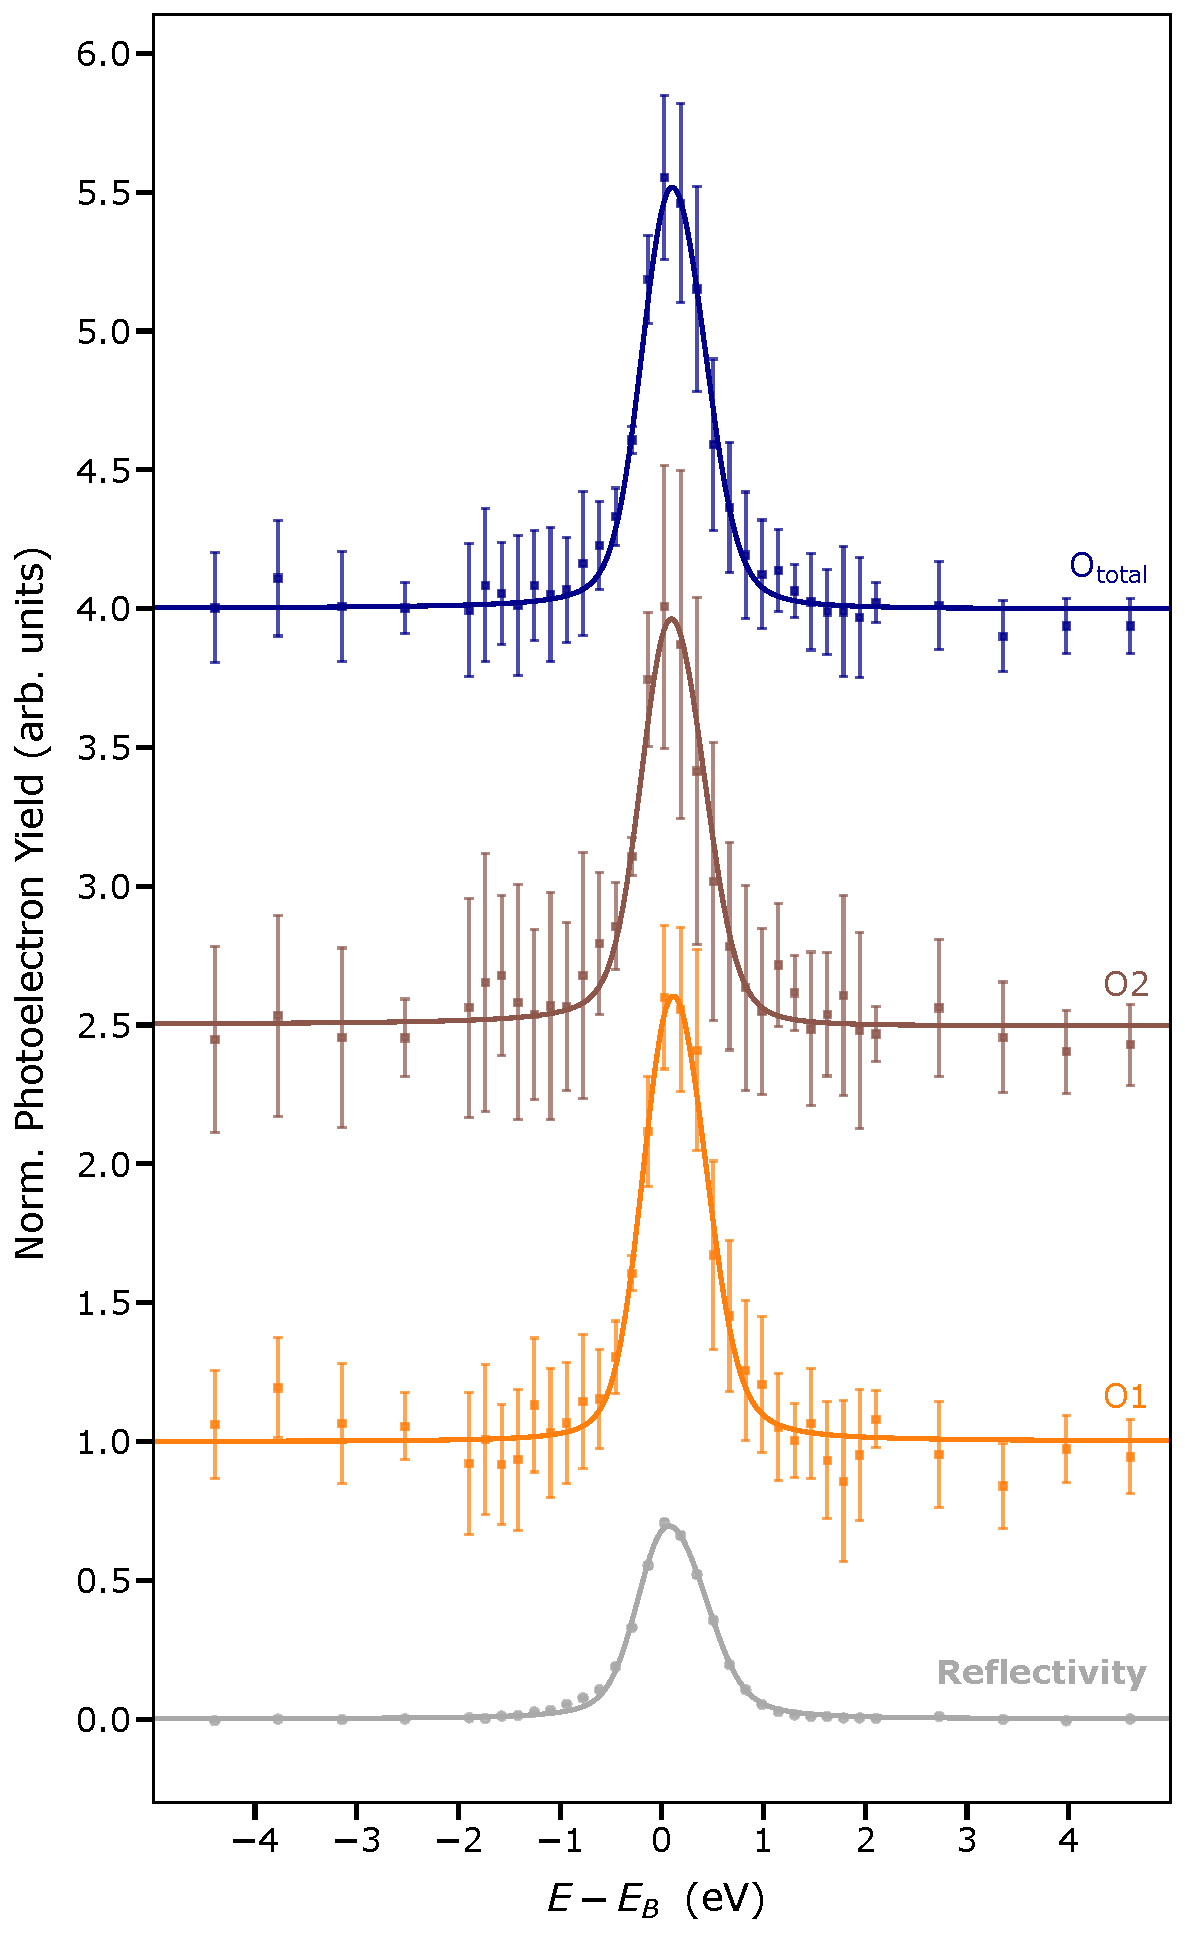
\includegraphics[width=0.75\linewidth]{images/NIXSW/NIXSW_O1s_Beta.pdf}
		\caption{$\beta$-phase}
	\end{subfigure}
\end{figure}

\end{frame}


%%%%%%%%%%%%%%
\begin{frame}
\frametitle{NIXSW: Comparison of the two phases}

\begin{figure}
	\centering
	\begin{subfigure}[t]{0.45\linewidth}
		\centering
		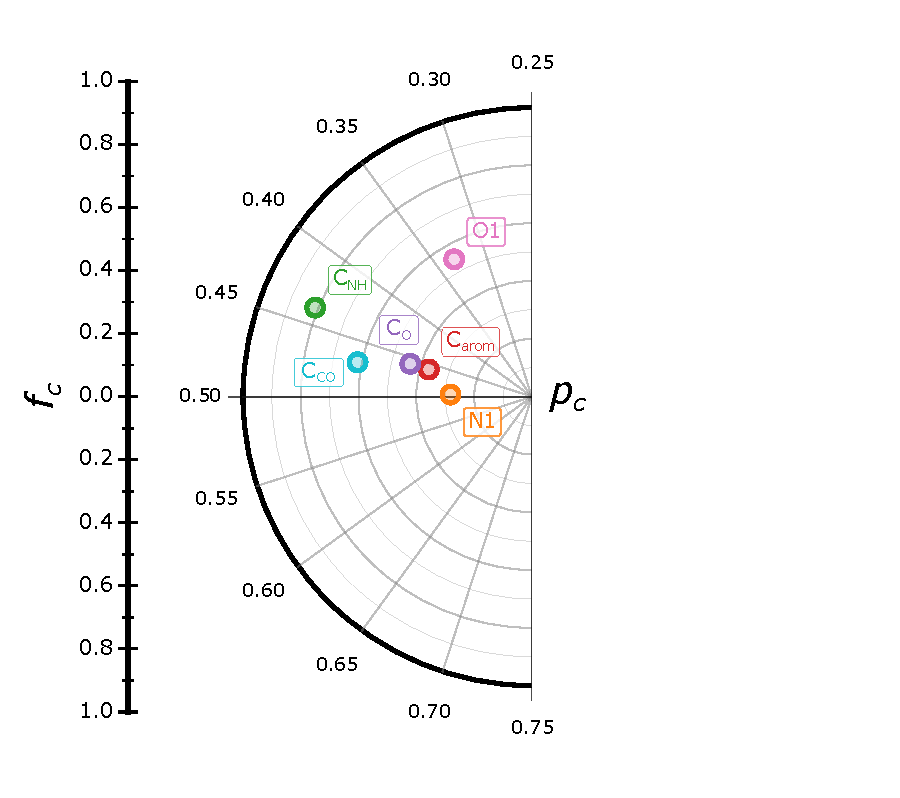
\includegraphics[height=\linewidth]{images/NIXSW/Argand_Alpha_2.pdf}
		\caption{$\alpha$-phase}
	\end{subfigure}
	\hfill
	\begin{subfigure}[t]{0.53\linewidth}
		\centering
		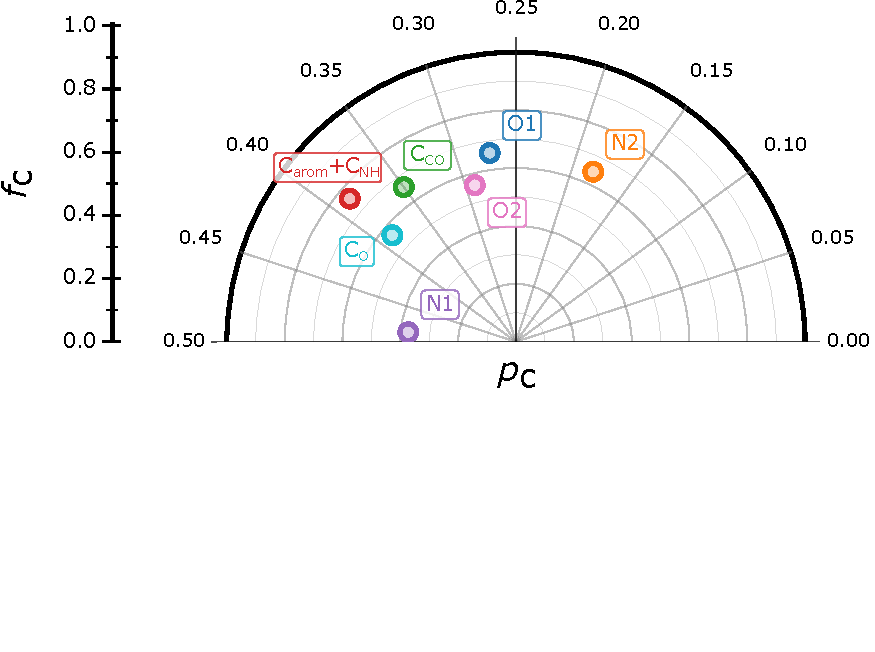
\includegraphics[width=\linewidth]{images/NIXSW/Argand_Beta_2.pdf}
		\caption{$\beta$-phase}
	\end{subfigure}
\end{figure}

\end{frame}


%%%%%%%%%%%%%%%%%%%%%%%%%%%%%%%%%%%%%%%%%%%%%%%%%%%%%%%%%%%%%%%%%%%
\section{Structure models of QA on Ag(100)}

\begin{frame}
\frametitle{$\alpha$-phase of QA on Ag(100)}

\begin{figure}
    \centering
    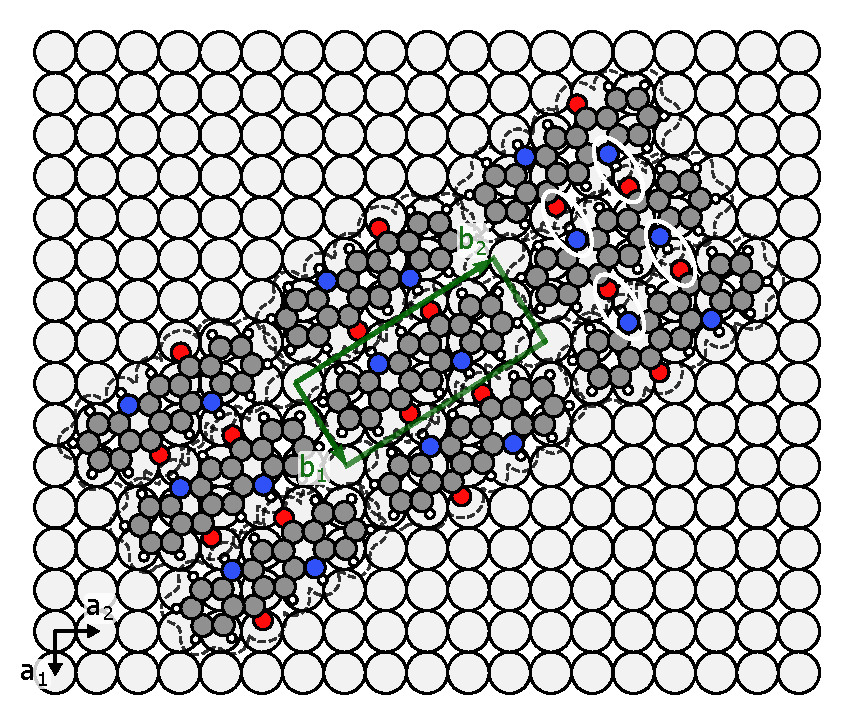
\includegraphics[width=0.75\textwidth]{images/Models/qa_alpha_top-view_with-vdw_9molecules.pdf}
\end{figure}

\end{frame}

%%%%%%%%%%%%%%
\begin{frame}
\frametitle{$\alpha$-phase of QA on Ag(100)}

\begin{figure}
	\centering
	\begin{subfigure}[b]{0.8\linewidth}
		\centering
		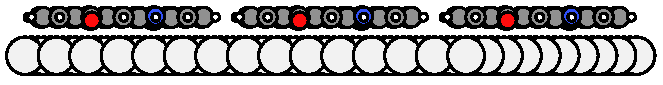
\includegraphics[width=\linewidth]{images/Models/qa_alpha_long-side_9molecules.pdf}
		\caption{Long side}
	\end{subfigure}

	\begin{subfigure}[b]{0.8\linewidth}
		\centering
		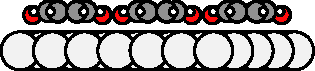
\includegraphics[width=\linewidth]{images/Models/qa_alpha_short-side_9molecules.pdf}
		\caption{Short side}
	\end{subfigure}
\end{figure}

\end{frame}

%%%%%%%%%%%%%%
\begin{frame}
\frametitle{$\beta$-phase of QA on Ag(100): Homochiral}

\begin{figure}
    \centering
    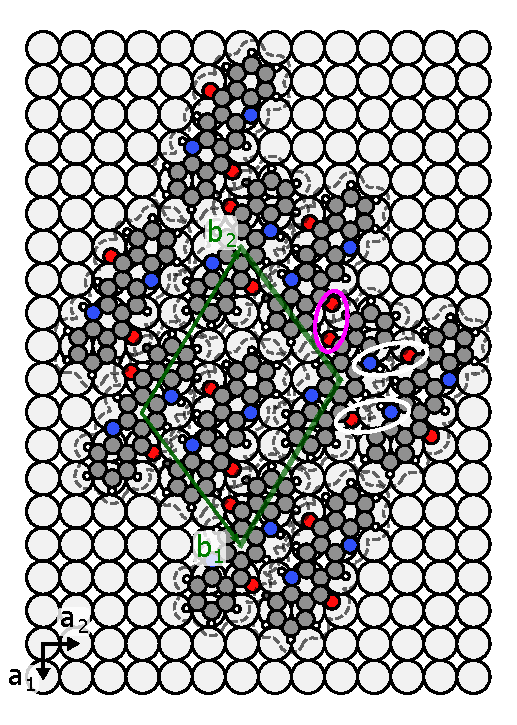
\includegraphics[width=0.48\textwidth]{images/Models/qa_beta_top-view_with_vdw_homochiral-10molecules.pdf}
\end{figure}

\end{frame}

%%%%%%%%%%%%%%
\begin{frame}
\frametitle{$\beta$-phase of QA on Ag(100): Homochiral}

\begin{figure}
	\centering
	\begin{subfigure}[b]{0.8\linewidth}
		\centering
		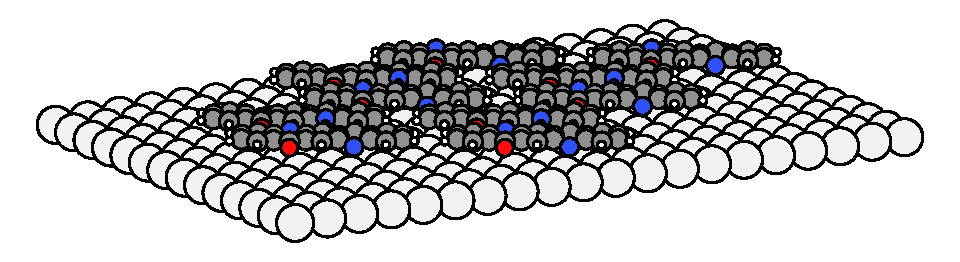
\includegraphics[width=\linewidth]{images/Models/qa_beta_long-side-slightly-up_homochiral-10molecules.pdf}
		\caption{Long side}
	\end{subfigure}

	\begin{subfigure}[b]{0.8\linewidth}
		\centering
		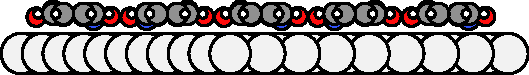
\includegraphics[width=\linewidth]{images/Models/qa_beta_short-side_homochiral-10molecules.pdf}
		\caption{Short side}
	\end{subfigure}
\end{figure}

\end{frame}

%%%%%%%%%%%%%%
\begin{frame}
\frametitle{$\beta$-phase of QA on Ag(100): Heterochiral}

\begin{figure}
    \centering
    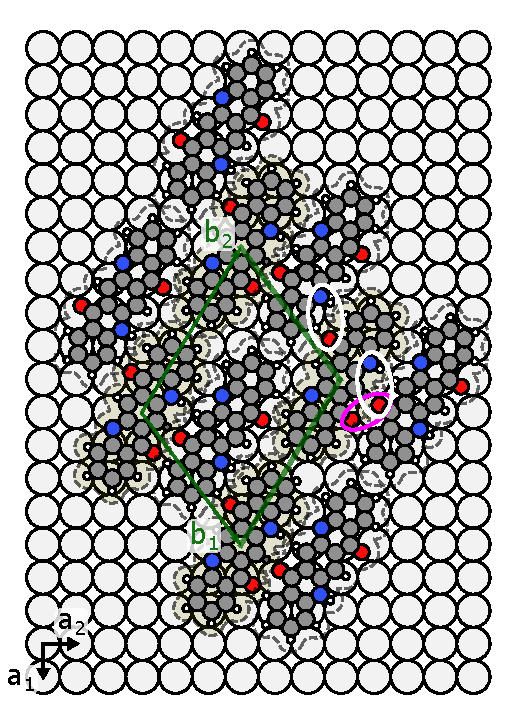
\includegraphics[width=0.48\textwidth]{images/Models/qa_beta_top-view_with_vdw_heterochiral-10molecules.pdf}
\end{figure}

\end{frame}

%%%%%%%%%%%%%%
\begin{frame}
\frametitle{$\beta$-phase of QA on Ag(100): Heterochiral}

\begin{figure}
	\centering
	\begin{subfigure}[b]{0.8\linewidth}
		\centering
		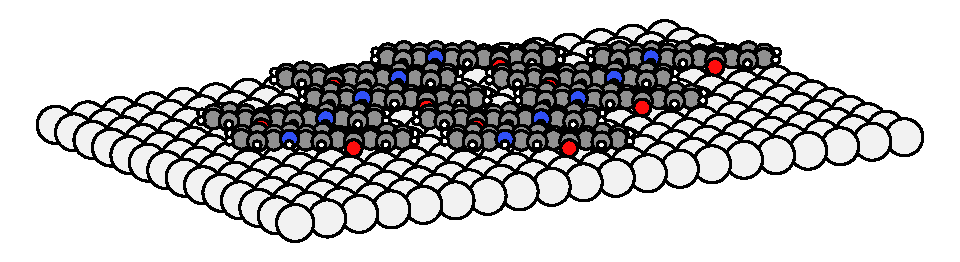
\includegraphics[width=\linewidth]{images/Models/qa_beta_long-side-slightly-up_heterochiral-10molecules.pdf}
		\caption{Long side}
	\end{subfigure}

	\begin{subfigure}[b]{0.8\linewidth}
		\centering
		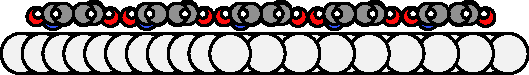
\includegraphics[width=\linewidth]{images/Models/qa_beta_short-side_heterochiral-10molecules.pdf}
		\caption{Short side}
	\end{subfigure}
\end{figure}

\end{frame}

%%%%%%%%%%%%%%
\begin{frame}
\frametitle{$\beta$-phase of QA on Ag(100): Dimers}

\begin{figure}
    \centering
    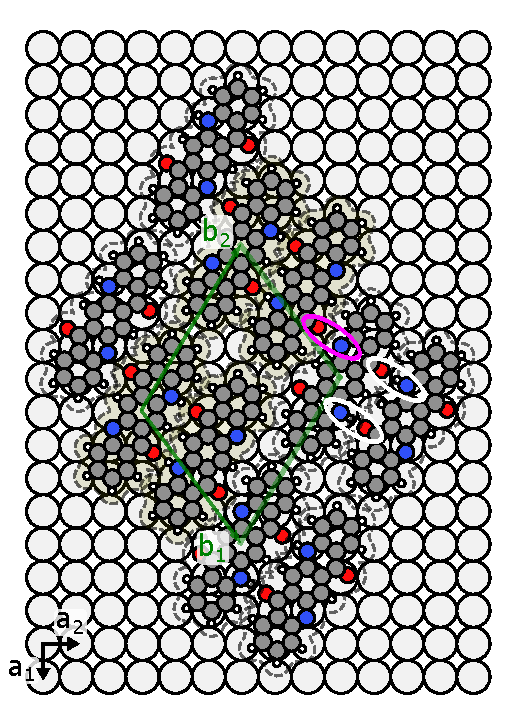
\includegraphics[width=0.48\textwidth]{images/Models/qa_beta_top-view_with_vdw_dimers-10molecules.pdf}
\end{figure}

\end{frame}

%%%%%%%%%%%%%%
\begin{frame}
\frametitle{$\beta$-phase of QA on Ag(100): Dimers}

\begin{figure}
	\centering
	\begin{subfigure}[b]{0.8\linewidth}
		\centering
		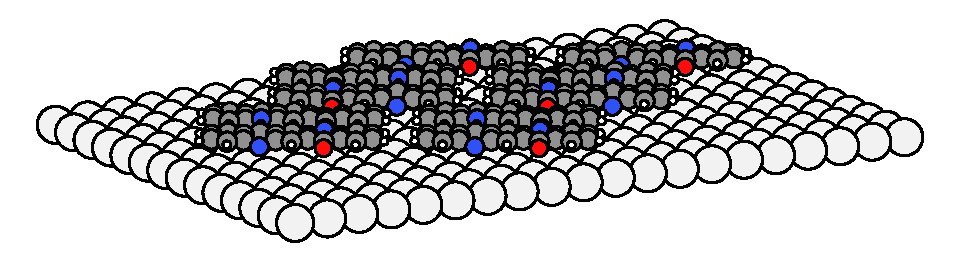
\includegraphics[width=\linewidth]{images/Models/qa_beta_long-side-slightly-up_dimers-10molecules.pdf}
		\caption{Long side}
	\end{subfigure}

	\begin{subfigure}[b]{0.8\linewidth}
		\centering
		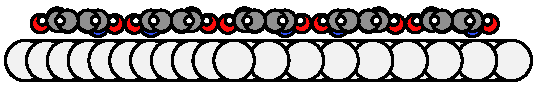
\includegraphics[width=\linewidth]{images/Models/qa_beta_short-side_dimers-10molecules.pdf}
		\caption{Short side}
	\end{subfigure}
\end{figure}

\end{frame}

%%%%%%%%%%%%%%%%%%%%%%%%%%%%%%%%%%%%%%%%%%%%%%%%%%%%%%%%%%%%%%%%%%%
\begin{frame}
\frametitle{References}
\begin{thebibliography}{99}
  \printbibliography[heading=bibliography]
\end{thebibliography}
\end{frame}

\begin{frame}
\frametitle{Thank you}
\centering
\huge
Questions?
\end{frame}

%%%%%%%%%%%%%%%%%%%%%%%%%%%%%%%%%%%%%%%%%%%%%%%%%%%%%%%%%%%%%%%%%%%
\appendix
\section{\appendixname}

\subsection{Multilayer}

%%%%%%%%%%%%%%
\begin{frame}
\frametitle{XPS: C1s Multilayer}

\begin{figure}
    \centering
    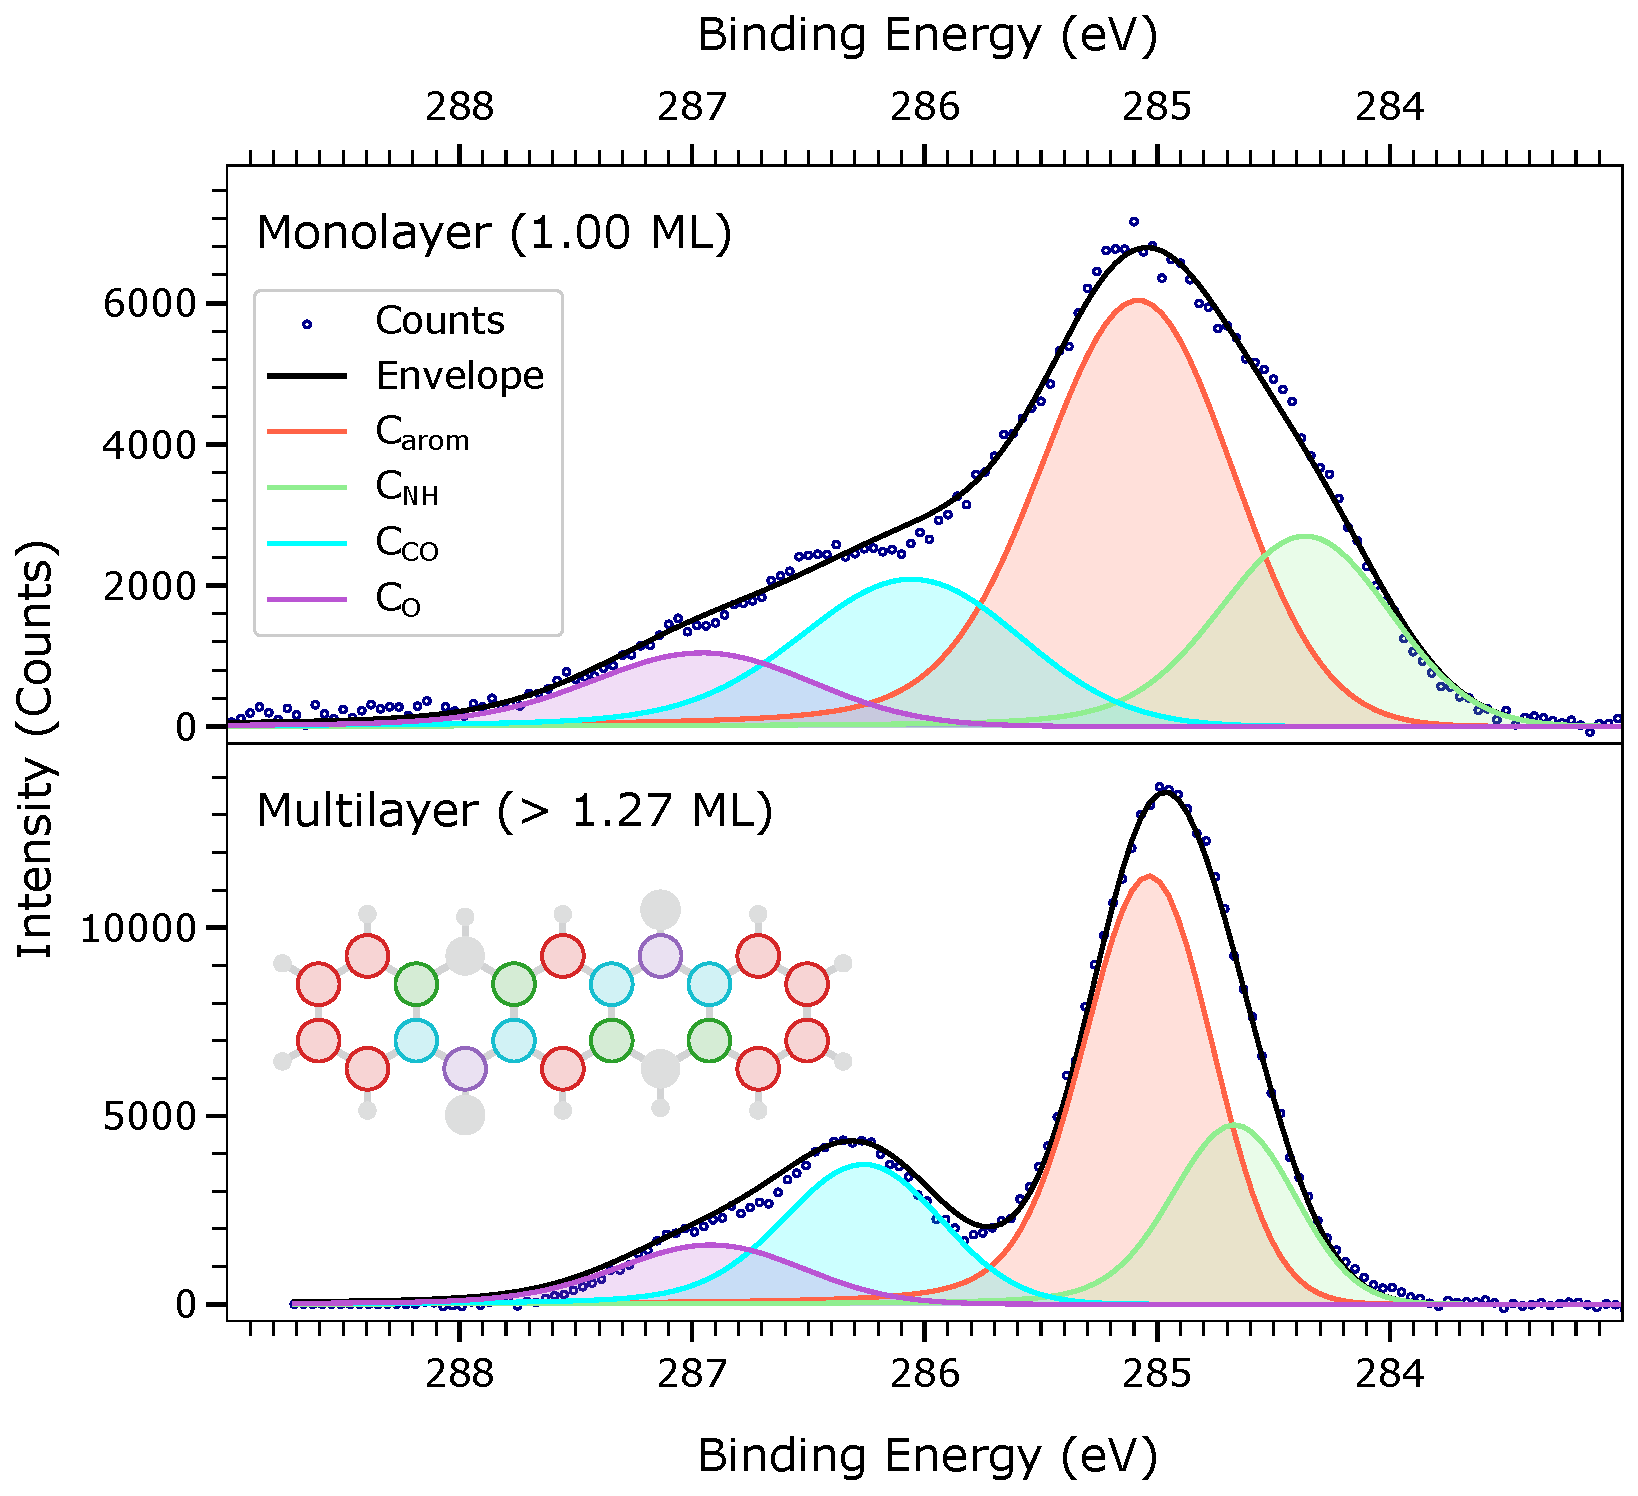
\includegraphics[width=0.7\textwidth]{images/XPS/C1s-Multilayer.pdf}
\end{figure}

\end{frame}

%%%%%%%%%%%%%%
\begin{frame}
\frametitle{XPS: N1s Multilayer}

\begin{figure}
    \centering
    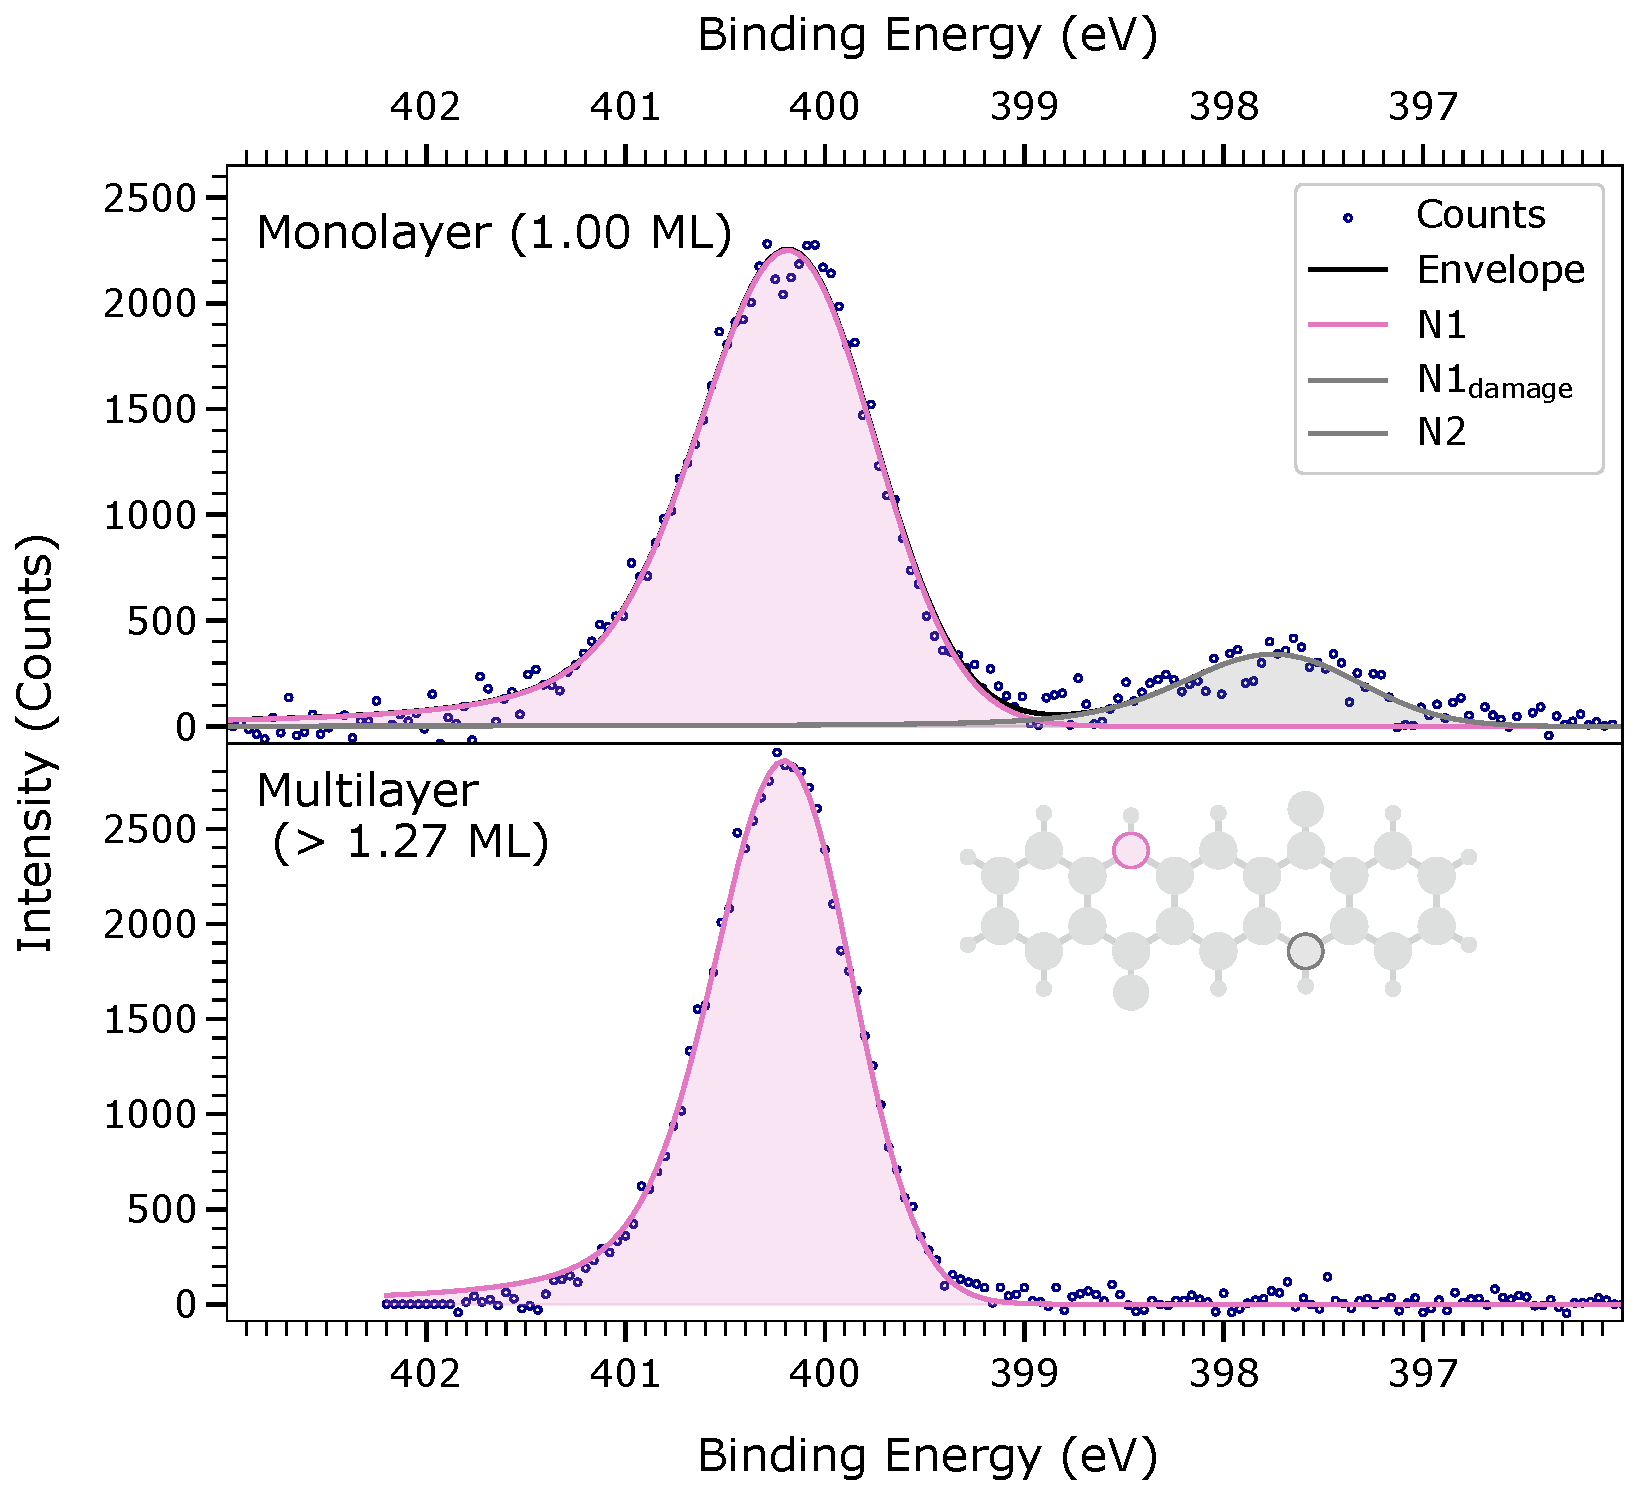
\includegraphics[width=0.7\textwidth]{images/XPS/N1s-Multilayer.pdf}
\end{figure}

\end{frame}

%%%%%%%%%%%%%%
\begin{frame}
\frametitle{XPS: O1s Multilayer}

\begin{figure}
    \centering
    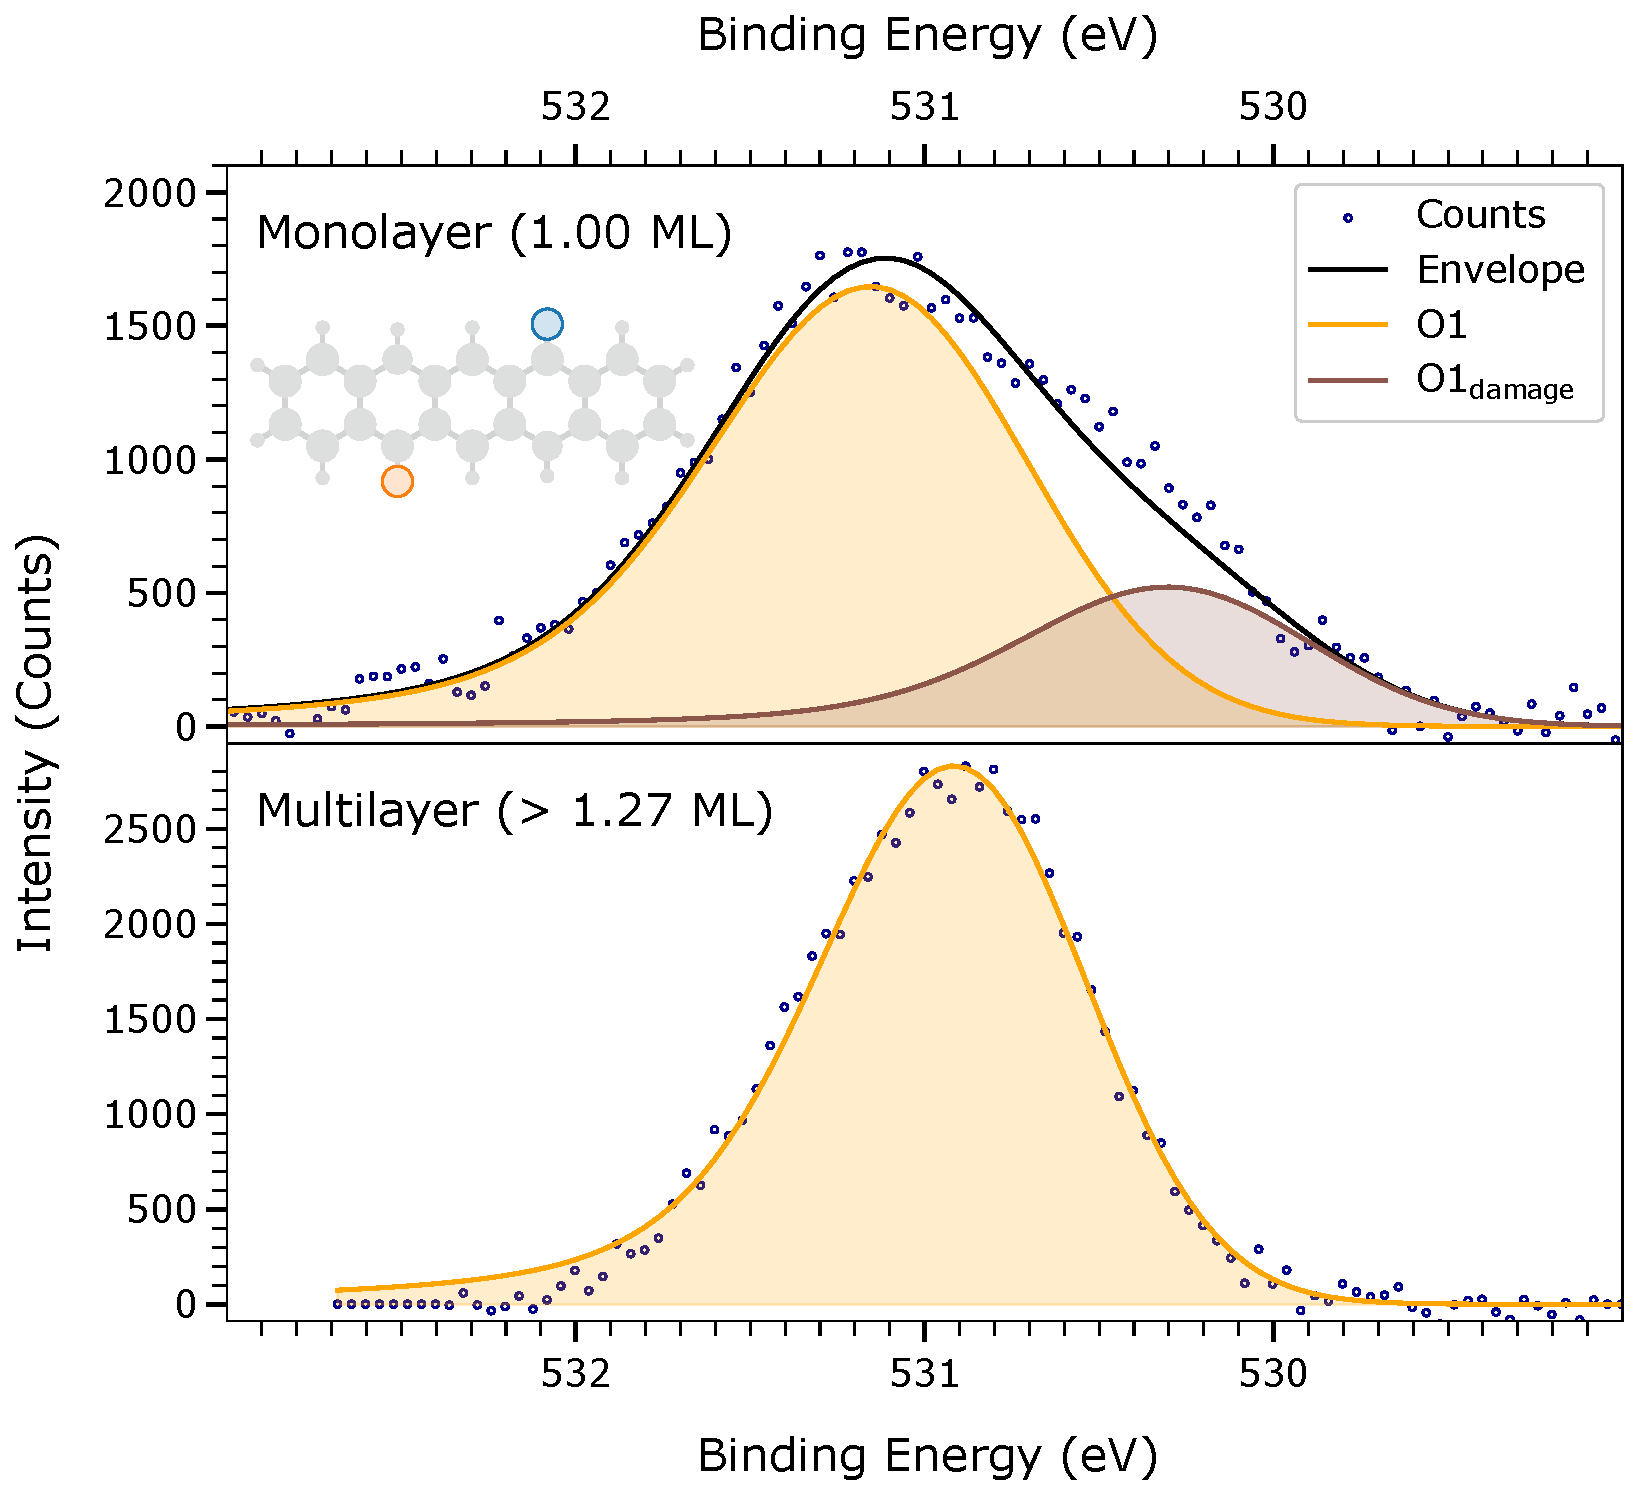
\includegraphics[width=0.7\textwidth]{images/XPS/O1s-Multilayer.pdf}
\end{figure}

\end{frame}


%%%%%%%%%%%%%%%%%%%%%%%%%%%%%%%%%%%%%%%%%%%%%%%%%%%%%%%%%%%%%%%%%%%
\subsection{Overview of all XPS spectra}

%%%%%%%%%%%%%%
\begin{frame}
\frametitle{XPS C1s}

\begin{figure}
    \centering
    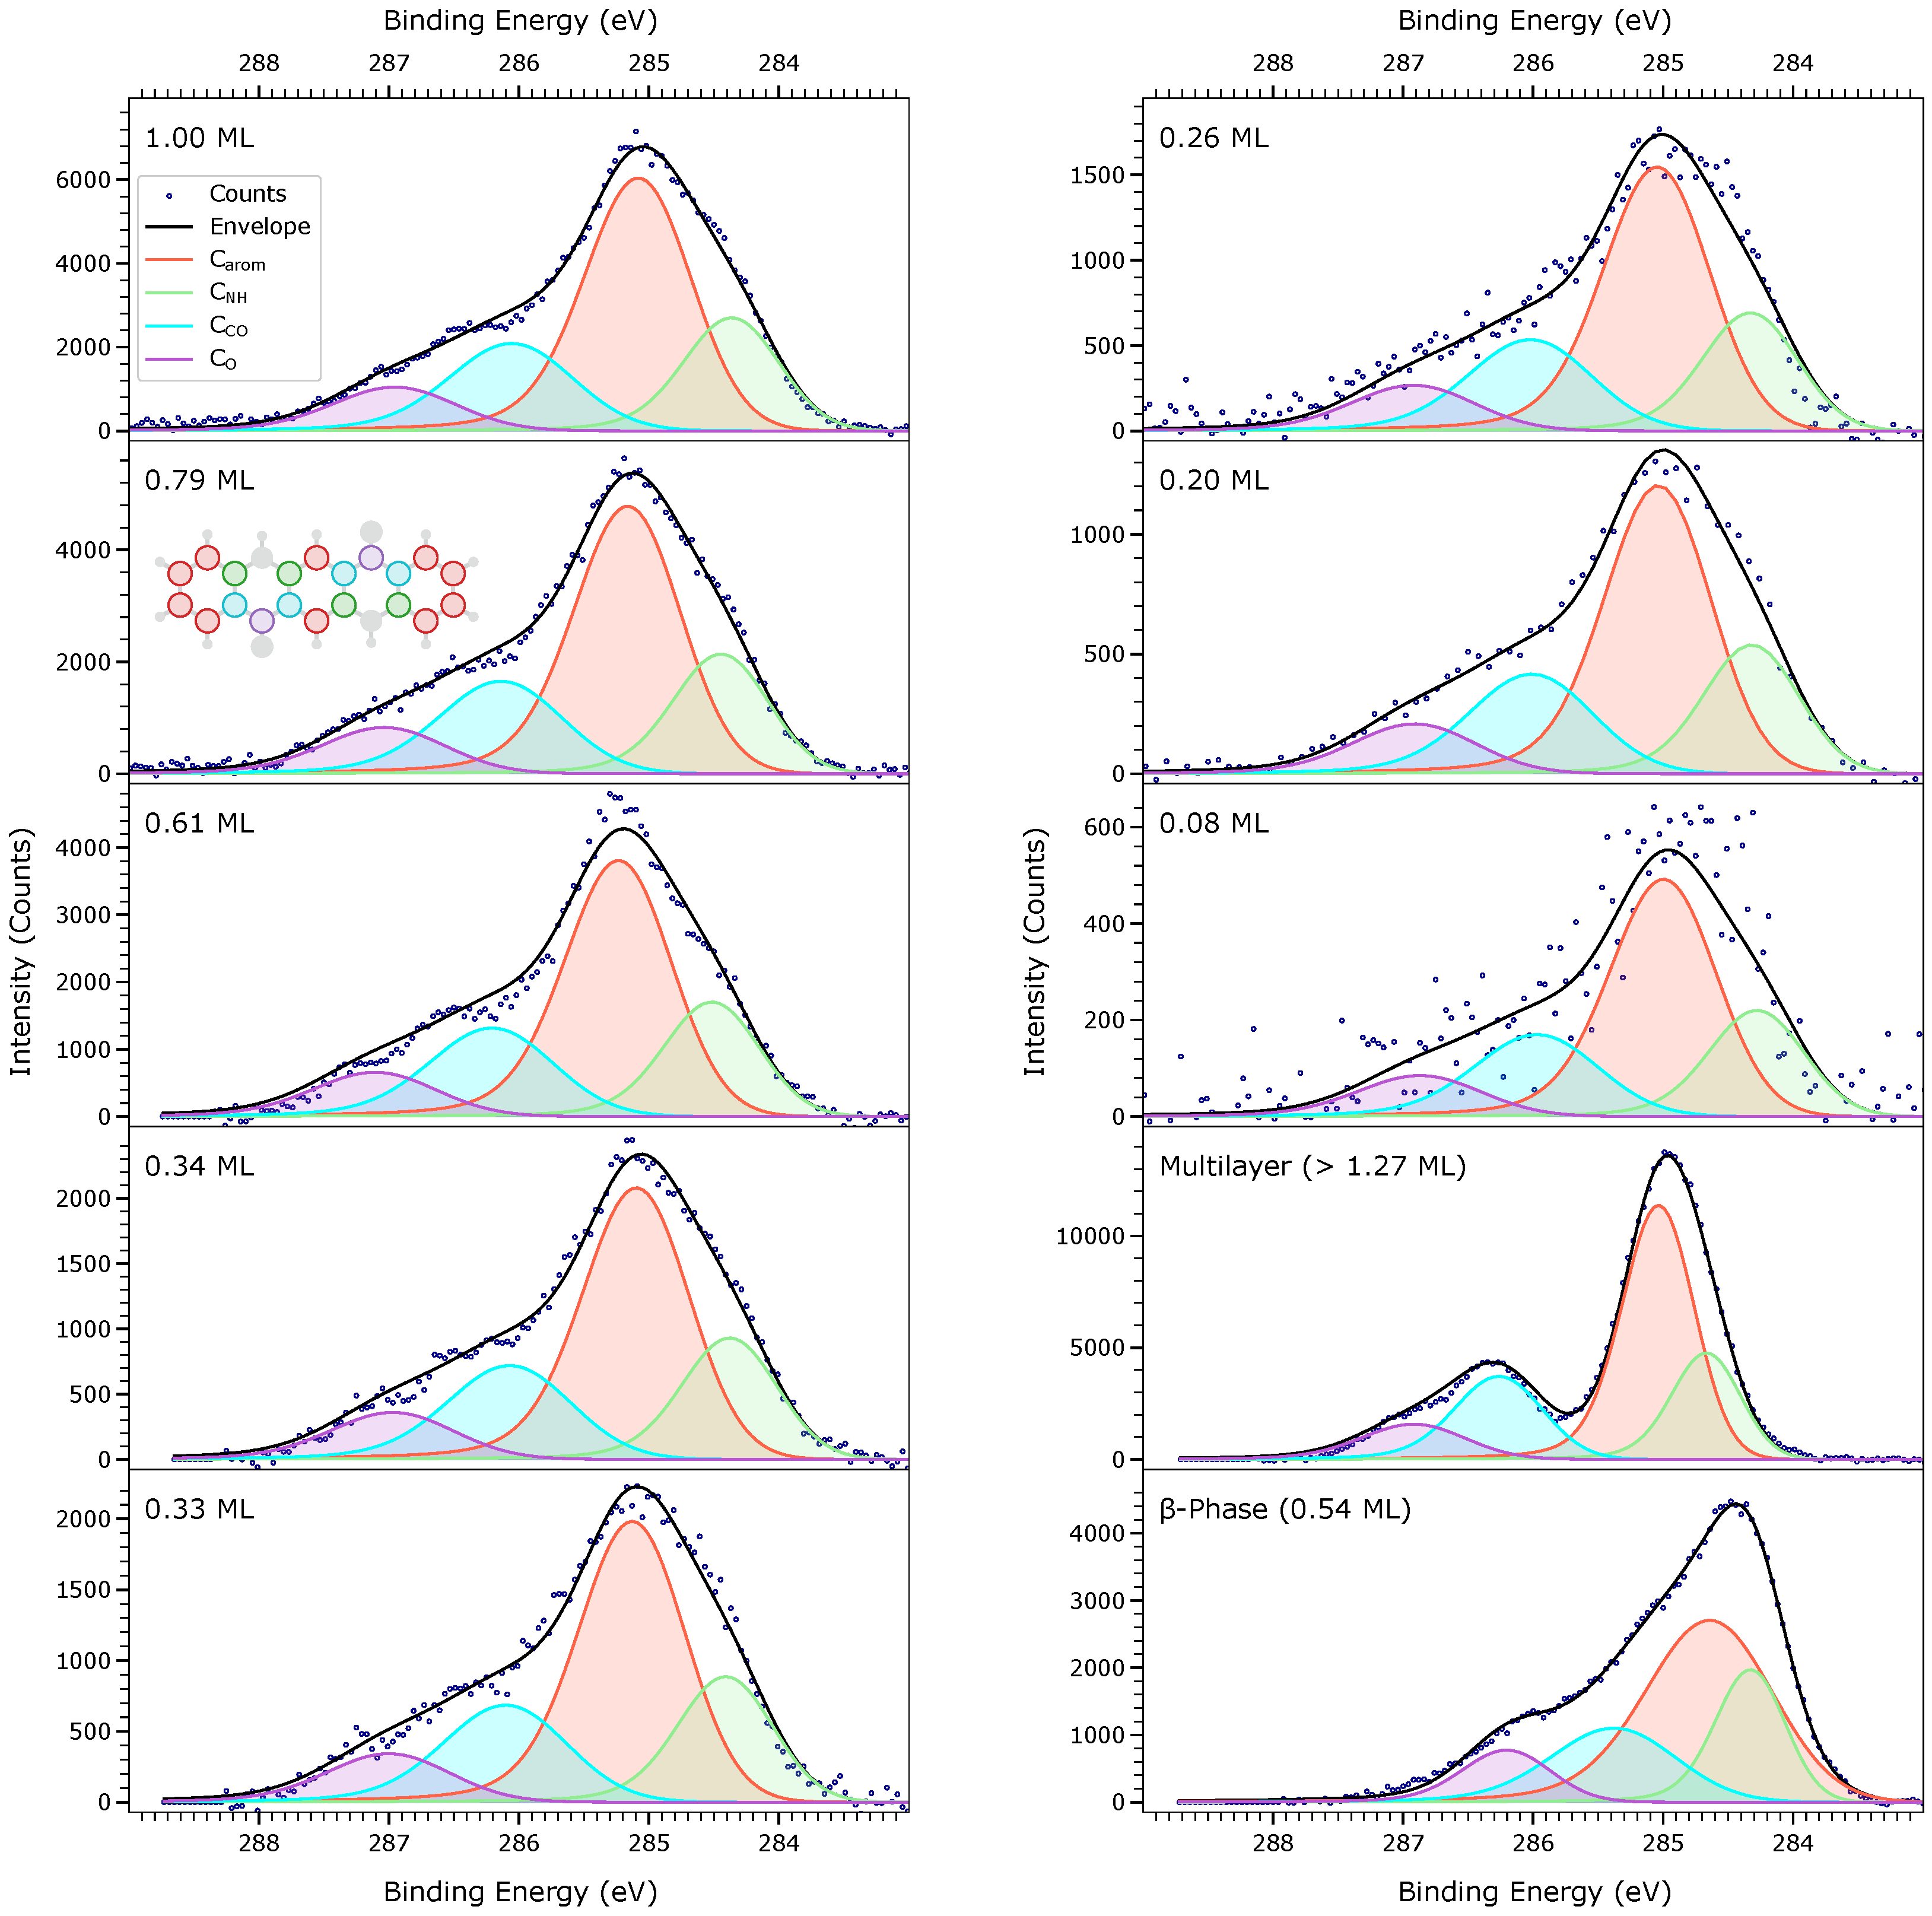
\includegraphics[width=0.65\textwidth]{images/XPS/C1s-All.pdf}
\end{figure}

\end{frame}

%%%%%%%%%%%%%%
\begin{frame}
\frametitle{XPS N1s}

\begin{figure}
    \centering
    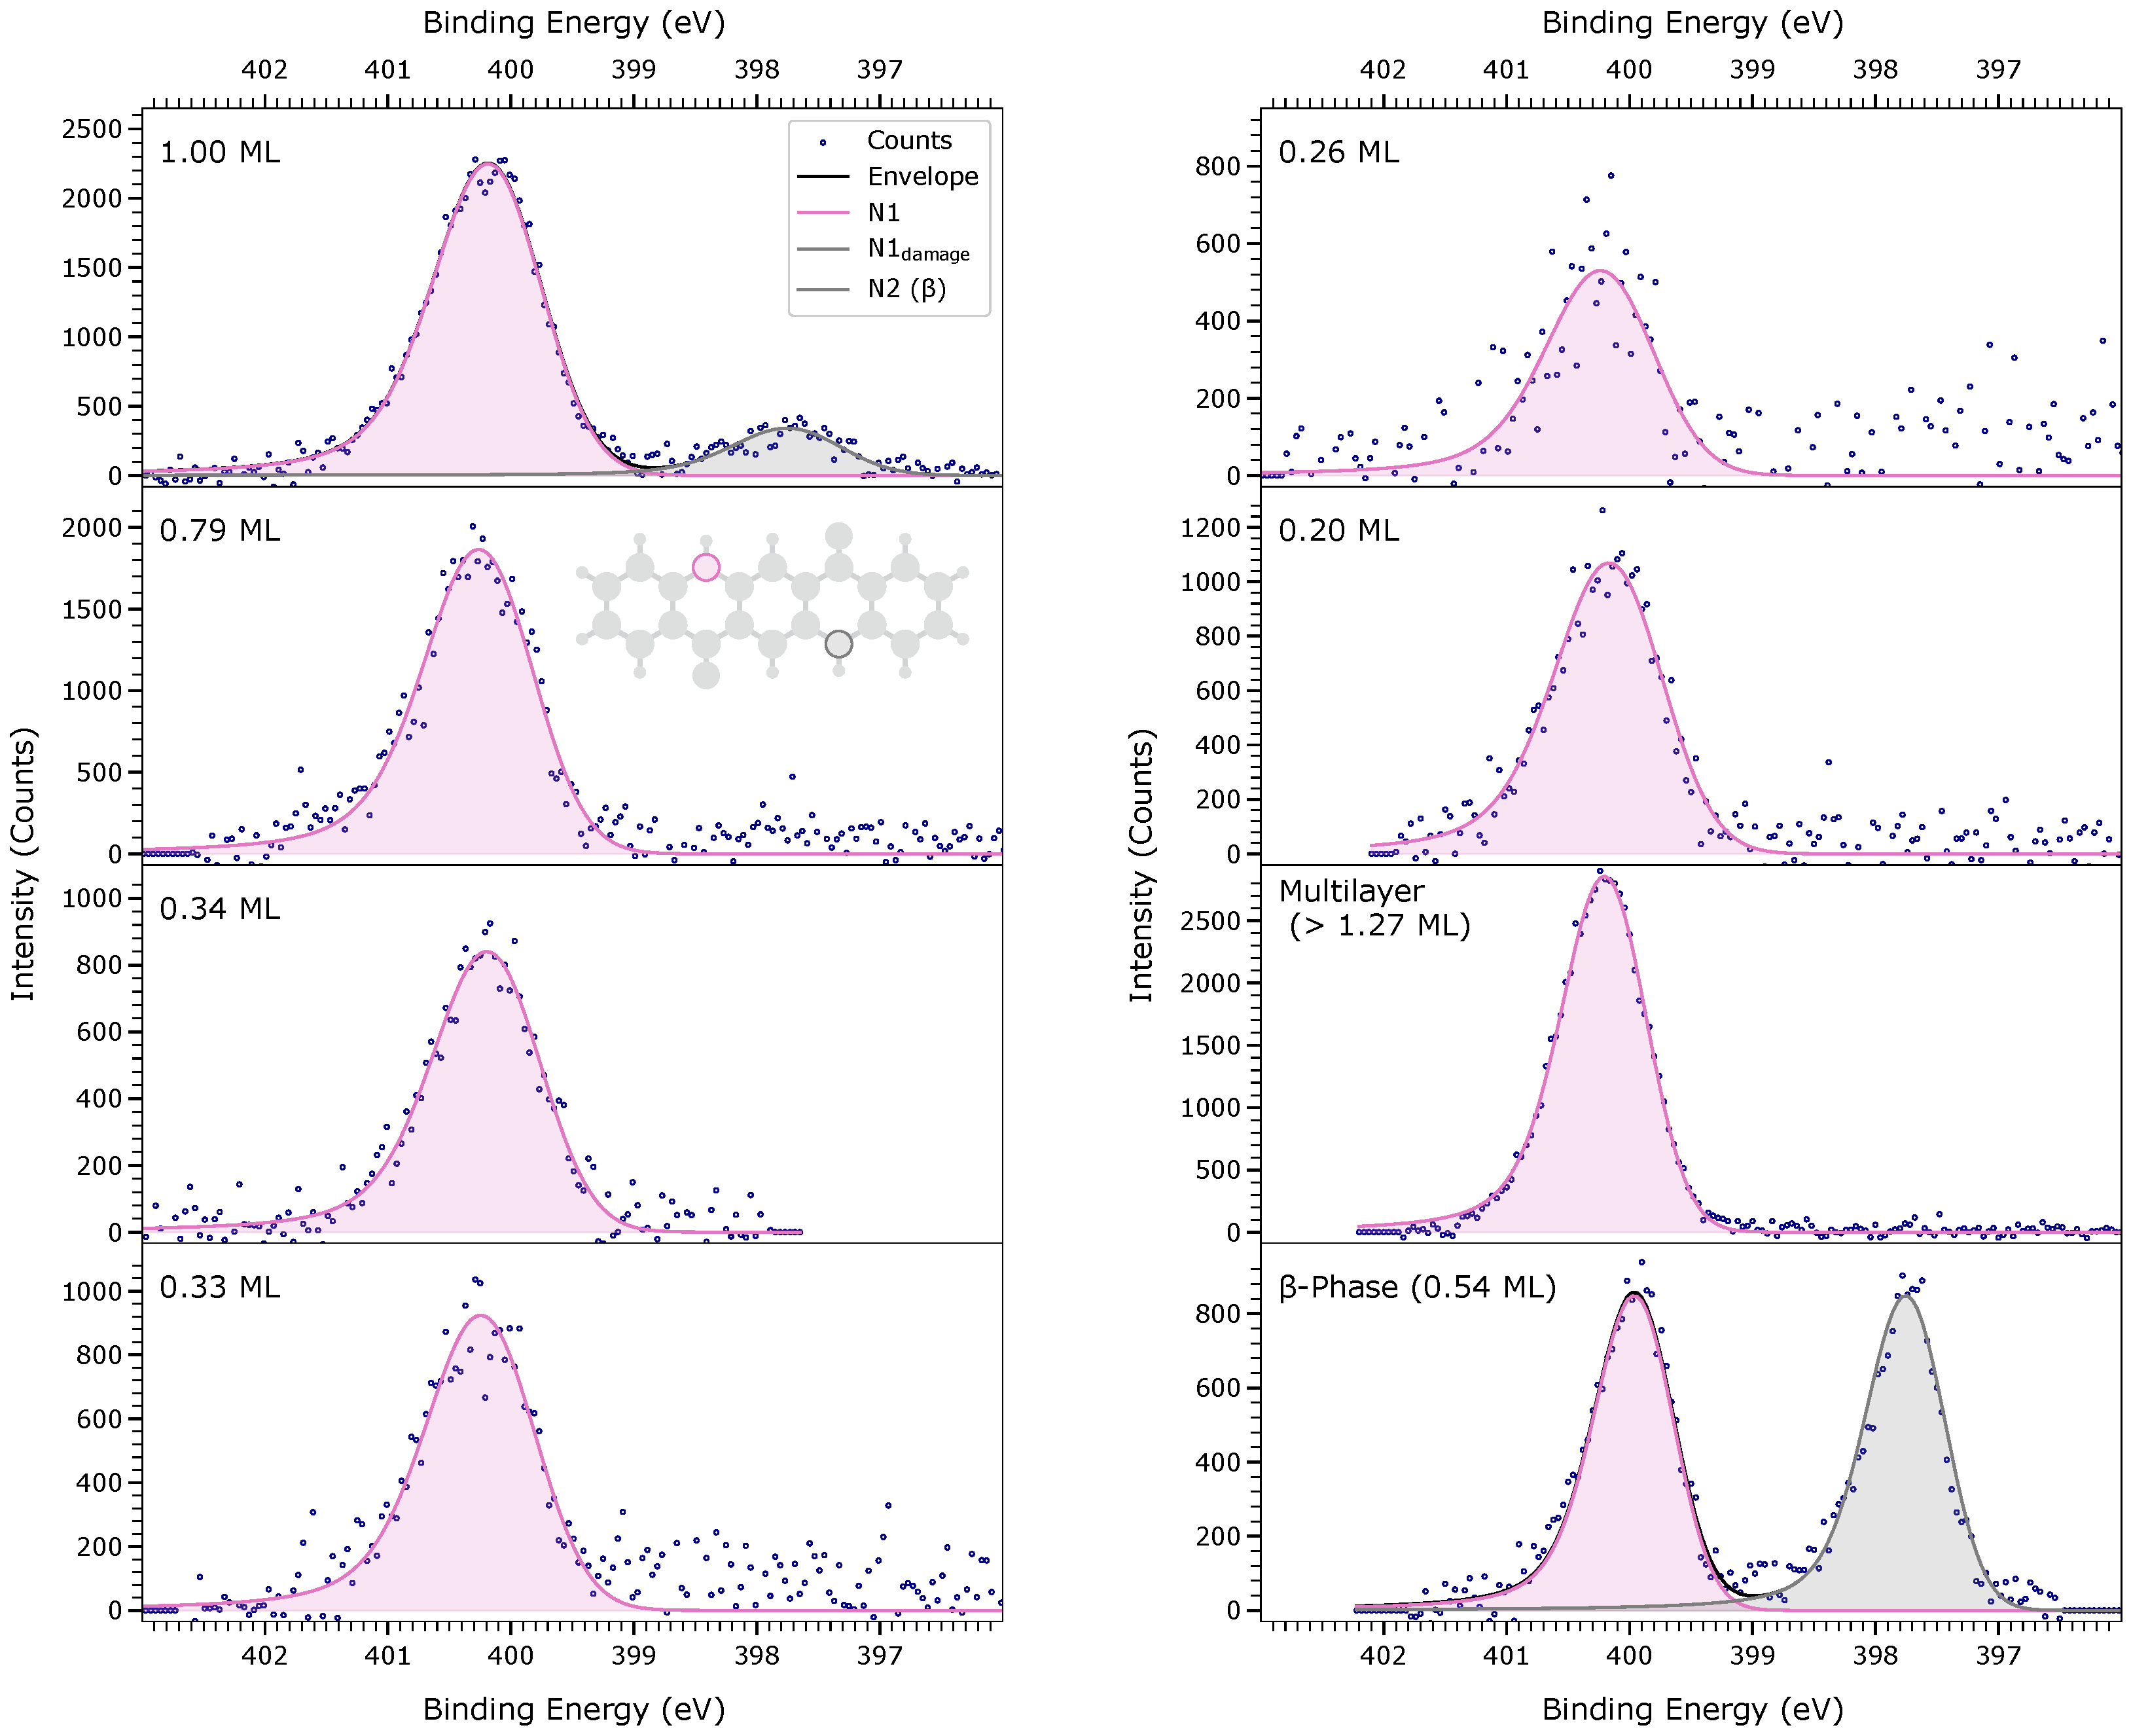
\includegraphics[width=0.8\textwidth]{images/XPS/N1s-All.pdf}
\end{figure}

\end{frame}

%%%%%%%%%%%%%%
\begin{frame}
\frametitle{XPS O1s}

\begin{figure}
    \centering
    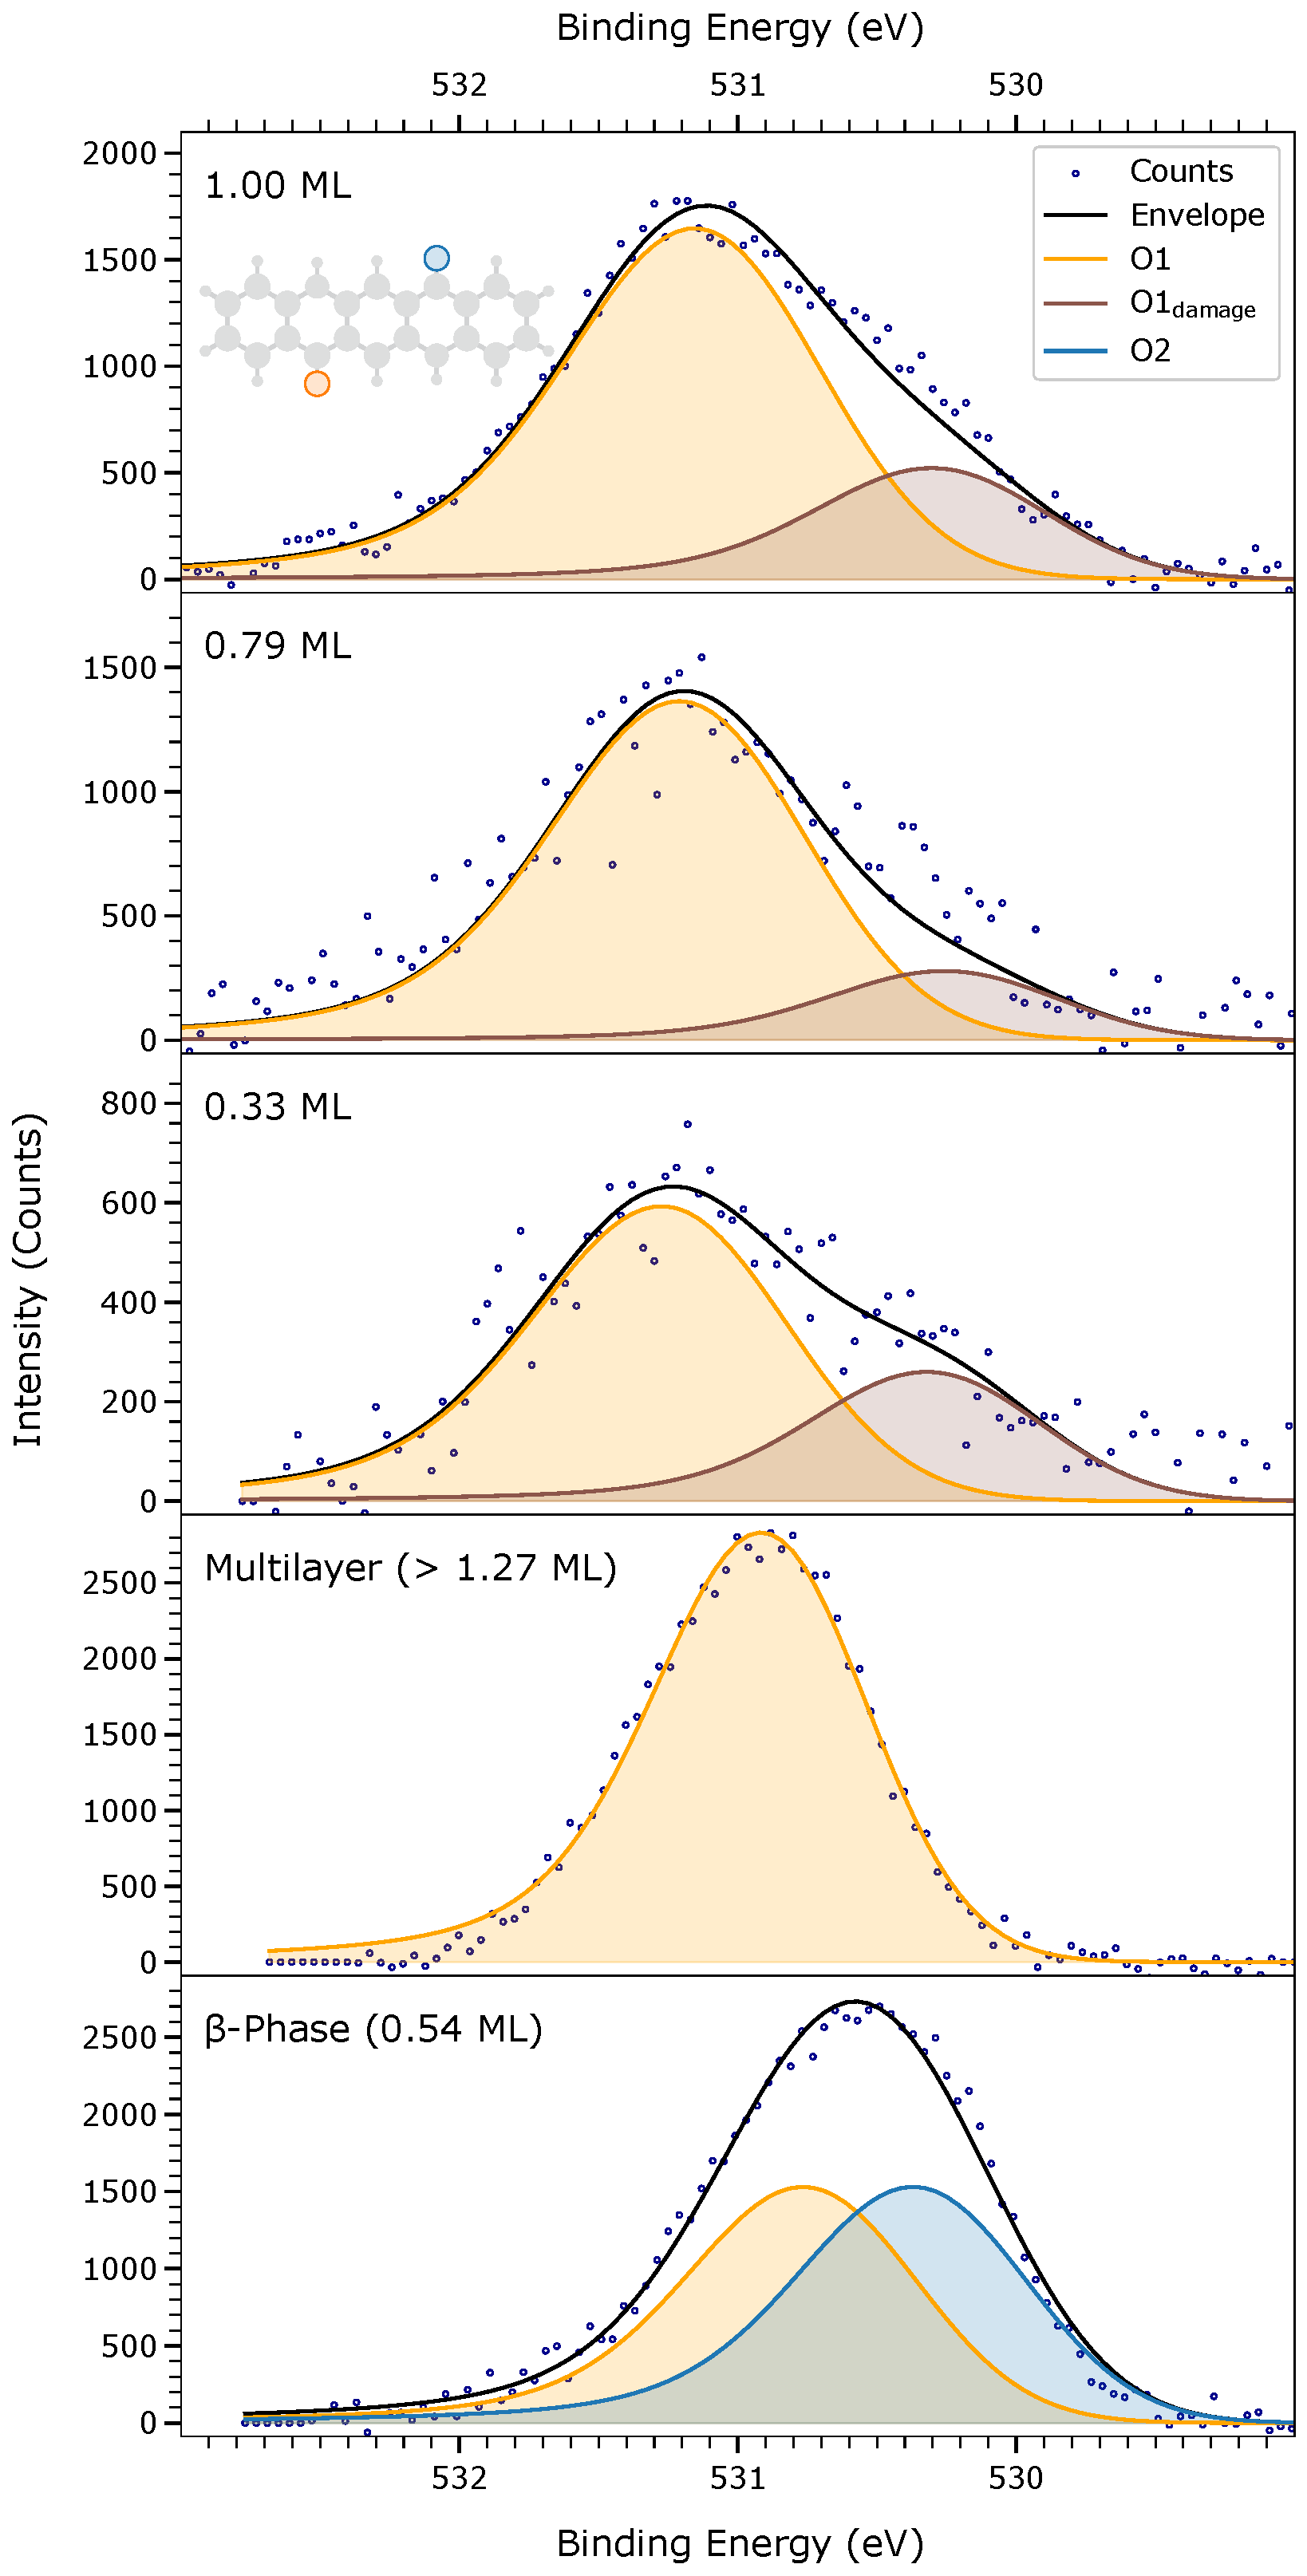
\includegraphics[width=0.3\textwidth]{images/XPS/O1s-All.pdf}
\end{figure}

\end{frame}

%%%%%%%%%%%%%%%%%%%%%%%%%%%%%%%%%%%%%%%%%%%%%%%%%%%%%%%%%%%%%%%%%%%
\subsection{Burnt Phase}

%%%%%%%%%%%%%%
\begin{frame}
\frametitle{XPS: C1s Multilayer}

\begin{figure}
    \centering
    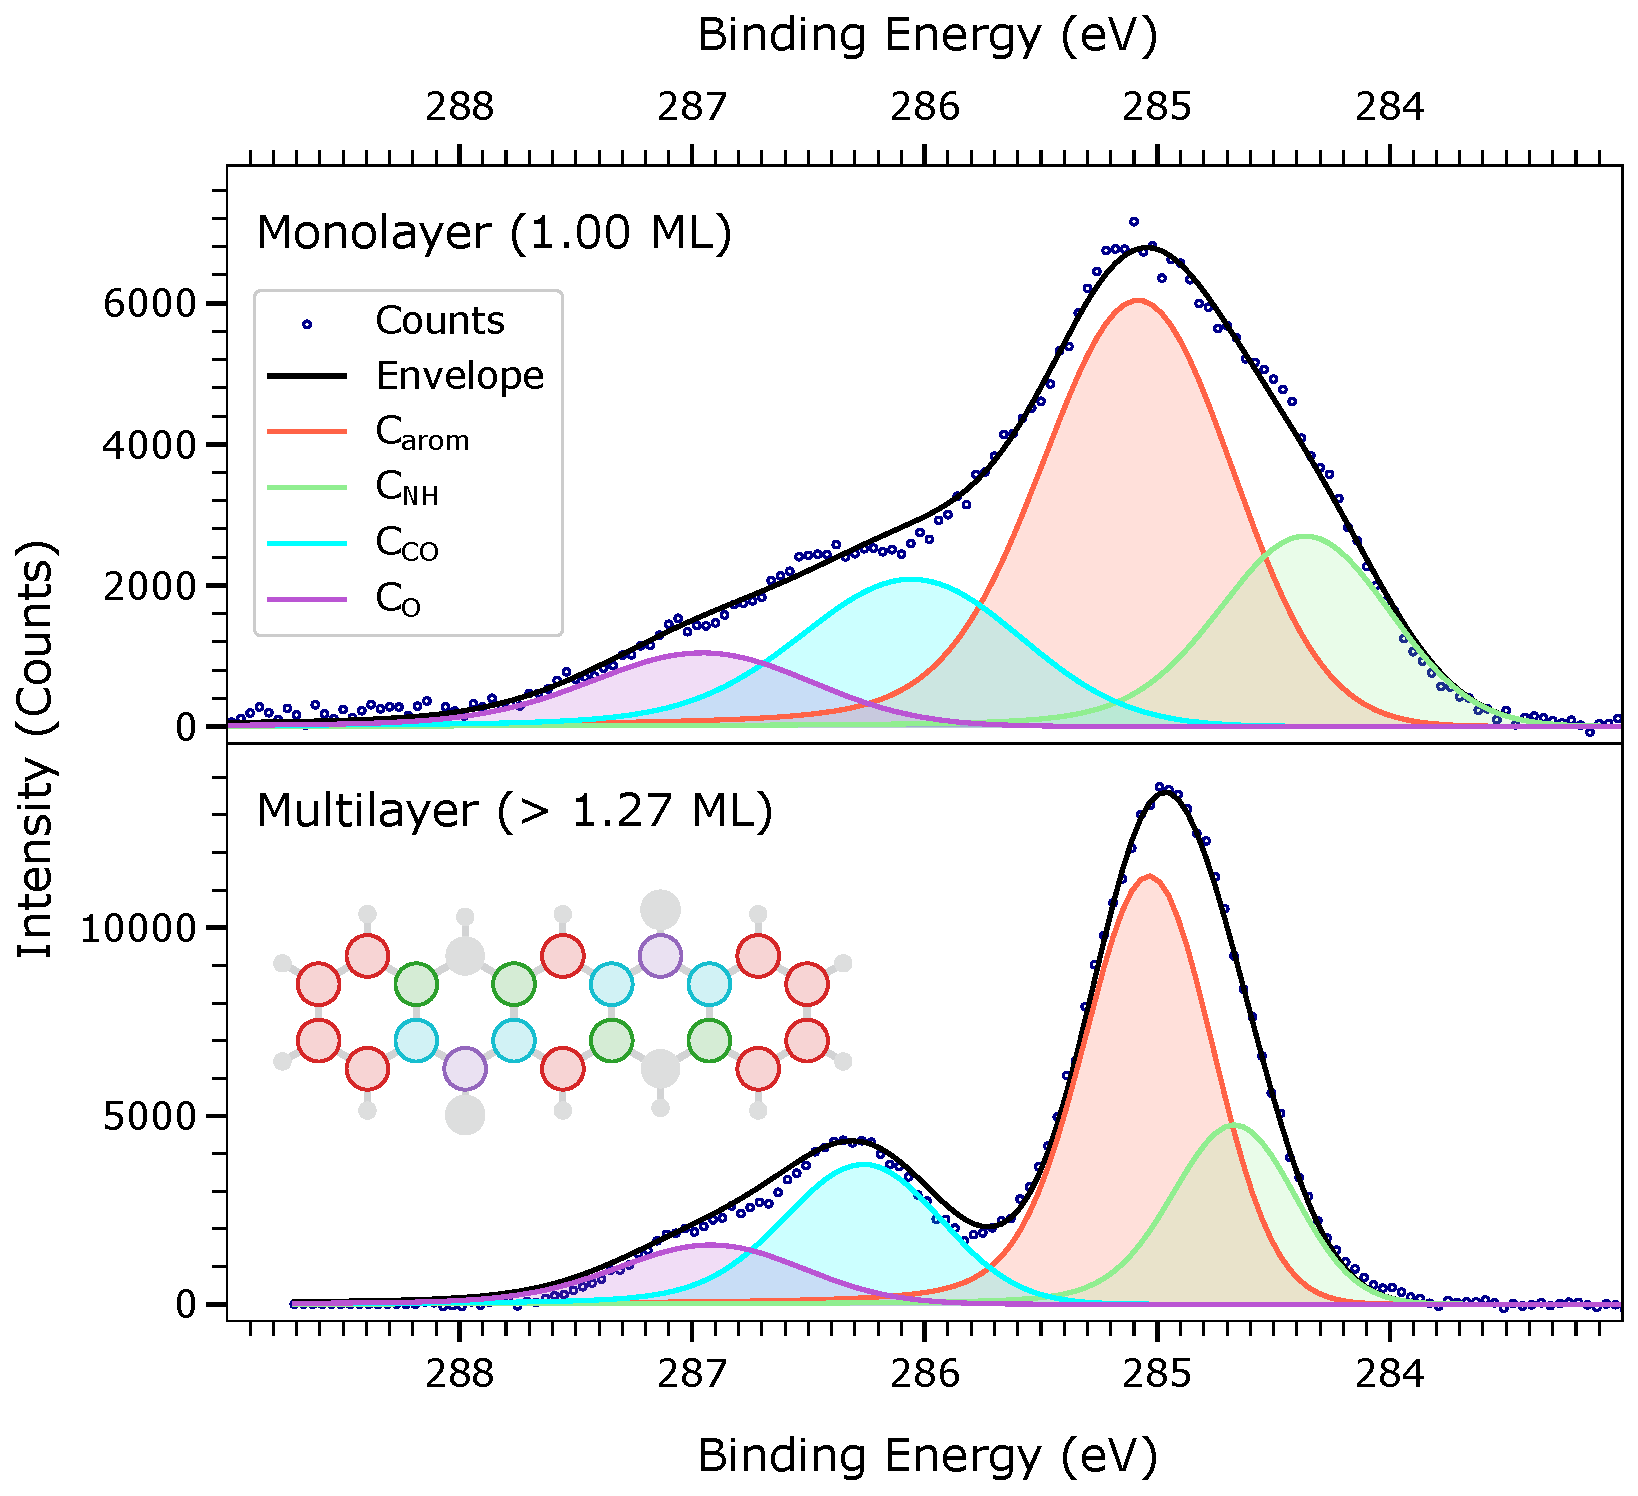
\includegraphics[width=0.7\textwidth]{images/XPS/C1s-Multilayer.pdf}
\end{figure}

\end{frame}

%%%%%%%%%%%%%%
\begin{frame}
\frametitle{XPS: C1s Burnt Phase}

\begin{figure}
    \centering
    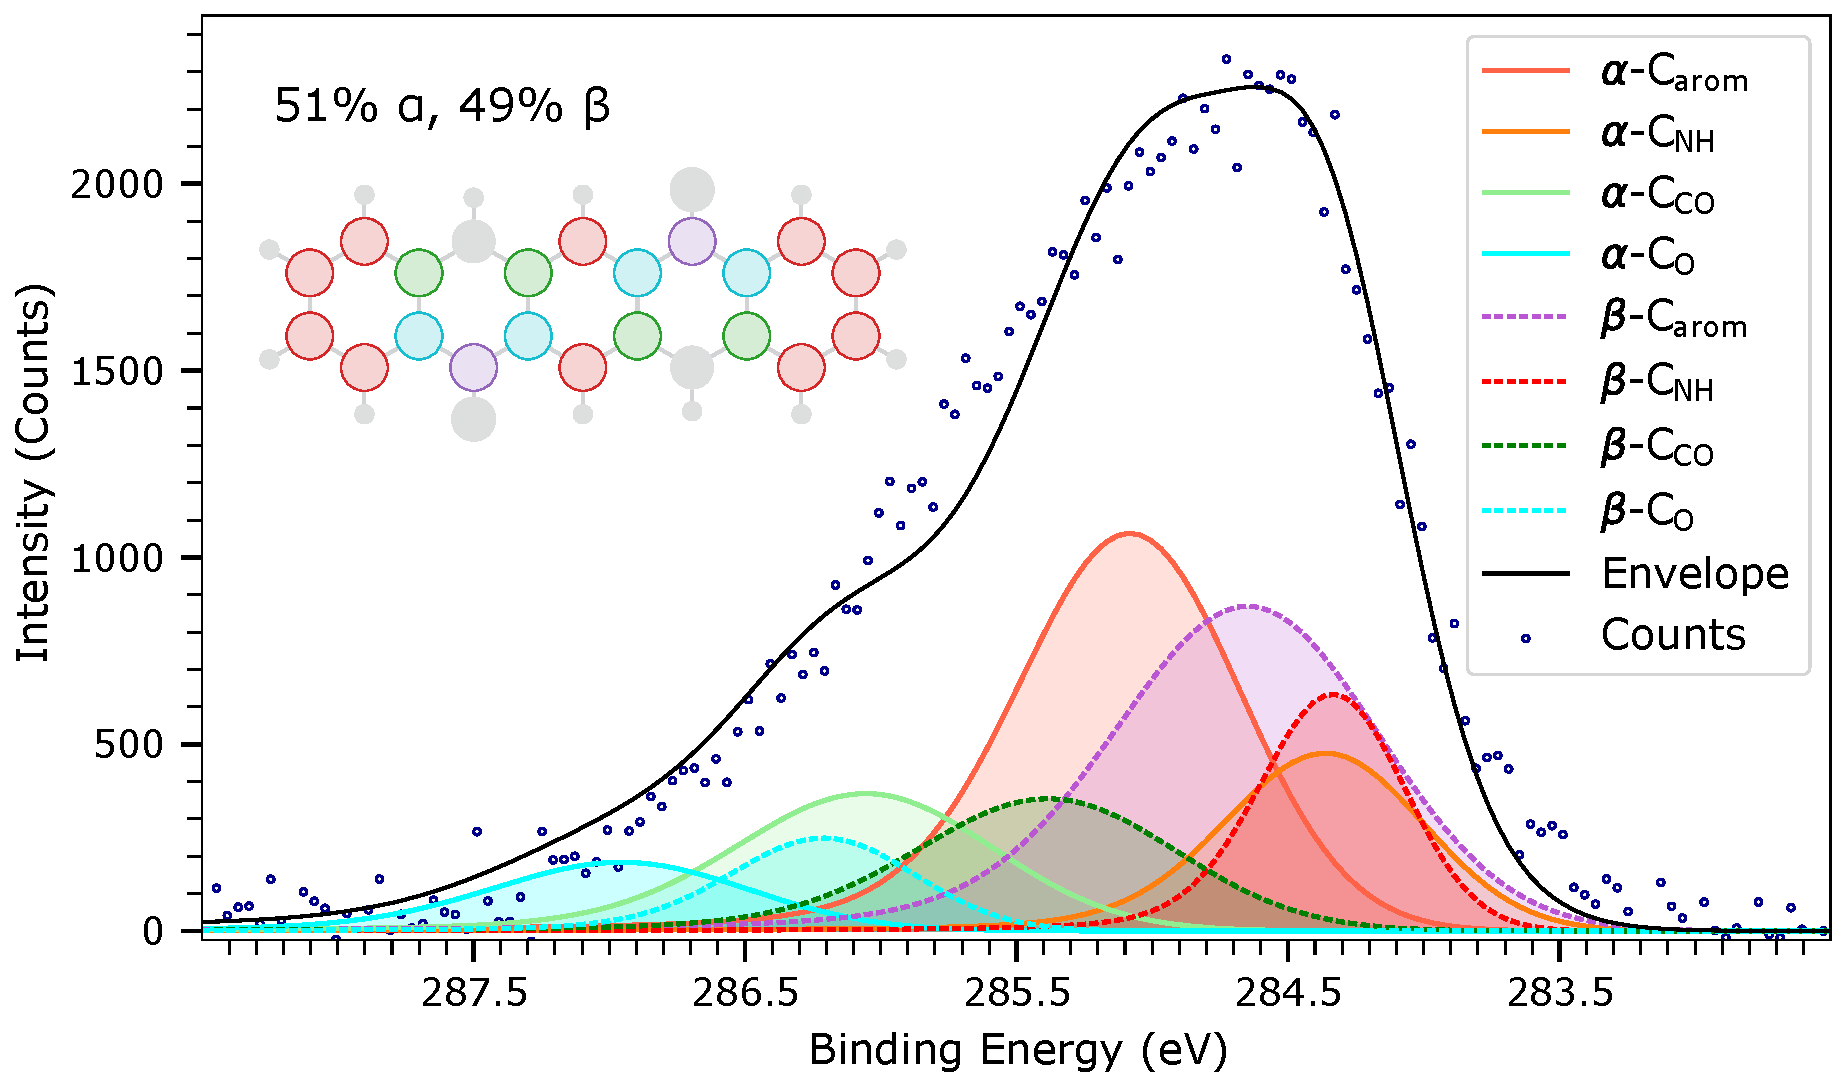
\includegraphics[width=0.8\textwidth]{images/XPS/C1s-BurntPhase.pdf}
\end{figure}

\end{frame}

%%%%%%%%%%%%%%
\begin{frame}
\frametitle{XPS: N1s Burnt Phase}

\begin{figure}
    \centering
    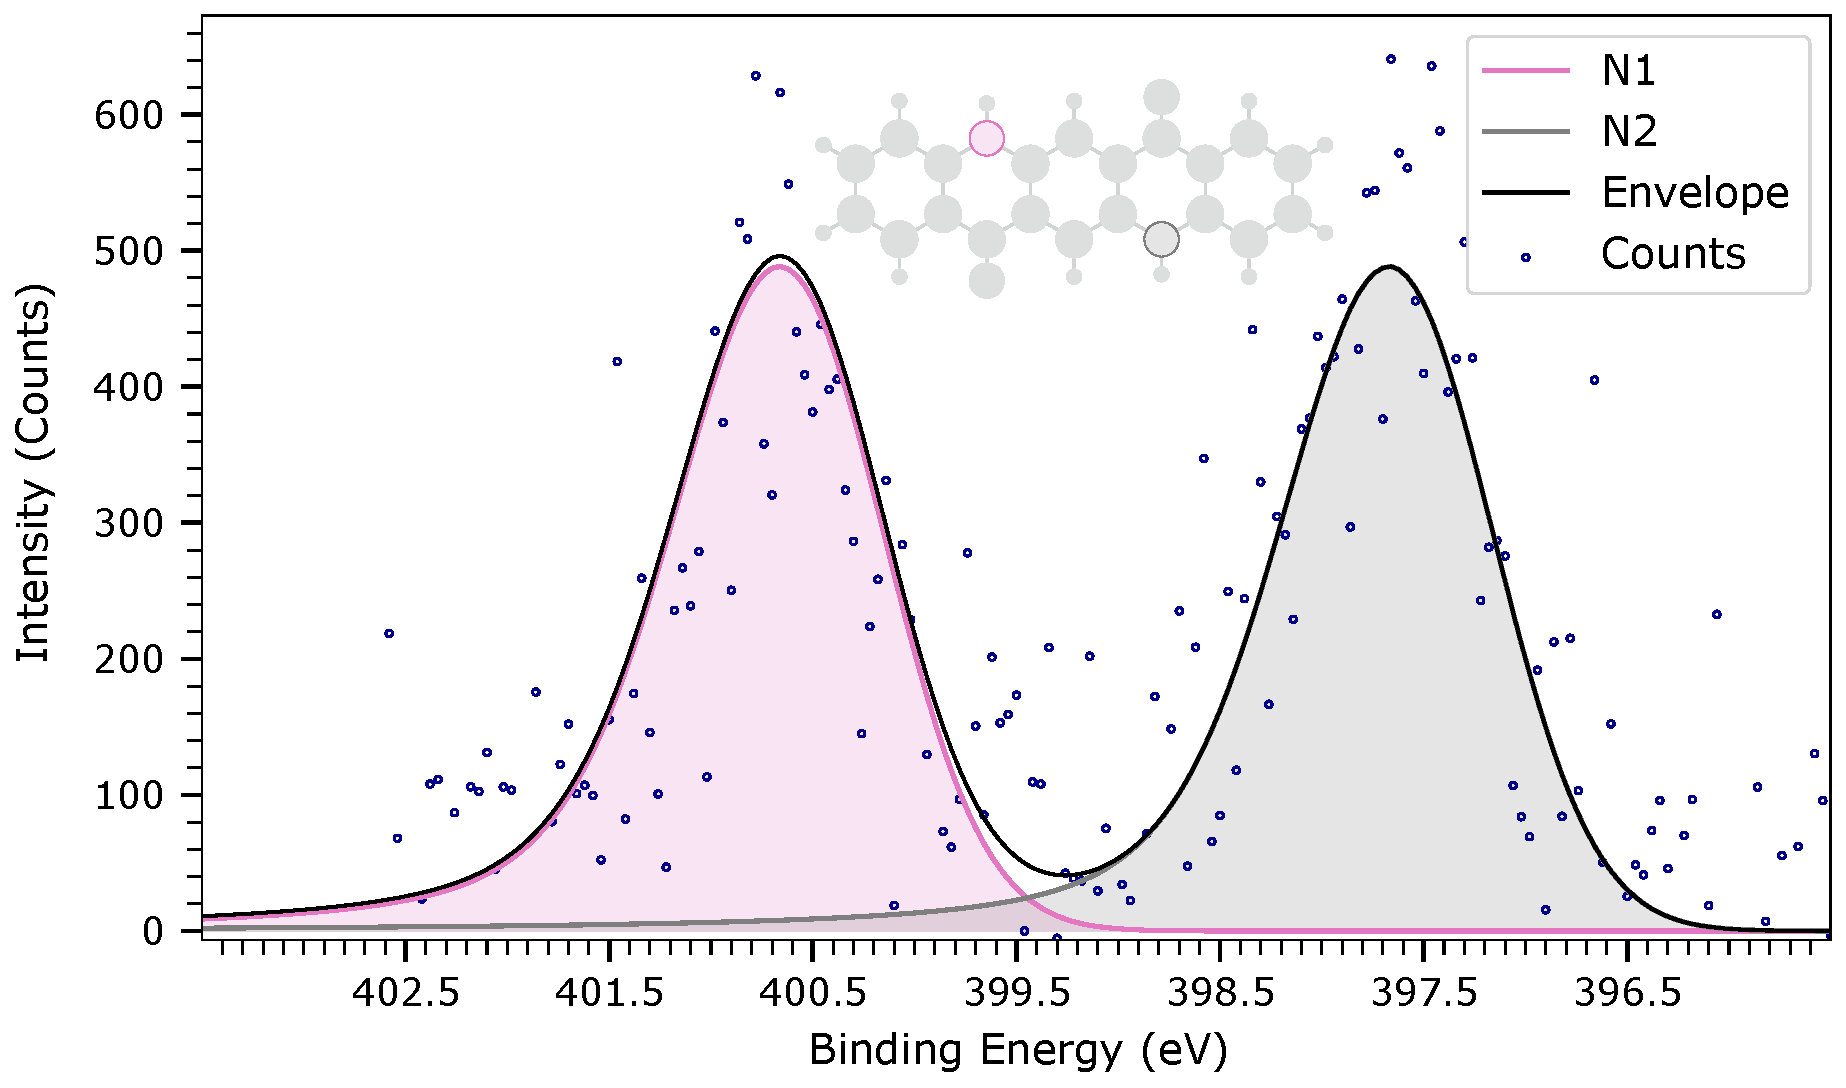
\includegraphics[width=0.8\textwidth]{images/XPS/N1s-BurntPhase.pdf}
\end{figure}

\end{frame}

%%%%%%%%%%%%%%%%%%%%%%%%%%%%%%%%%%%%%%%%%%%%%%%%%%%%%%%%%%%%%%%%%%%
\subsection{NIXSW Fit Model 3 Peaks}

%%%%%%%%%%%%%%
\begin{frame}
\frametitle{NIXSW Fit Model 3 Peaks}

\begin{figure}
    \centering
    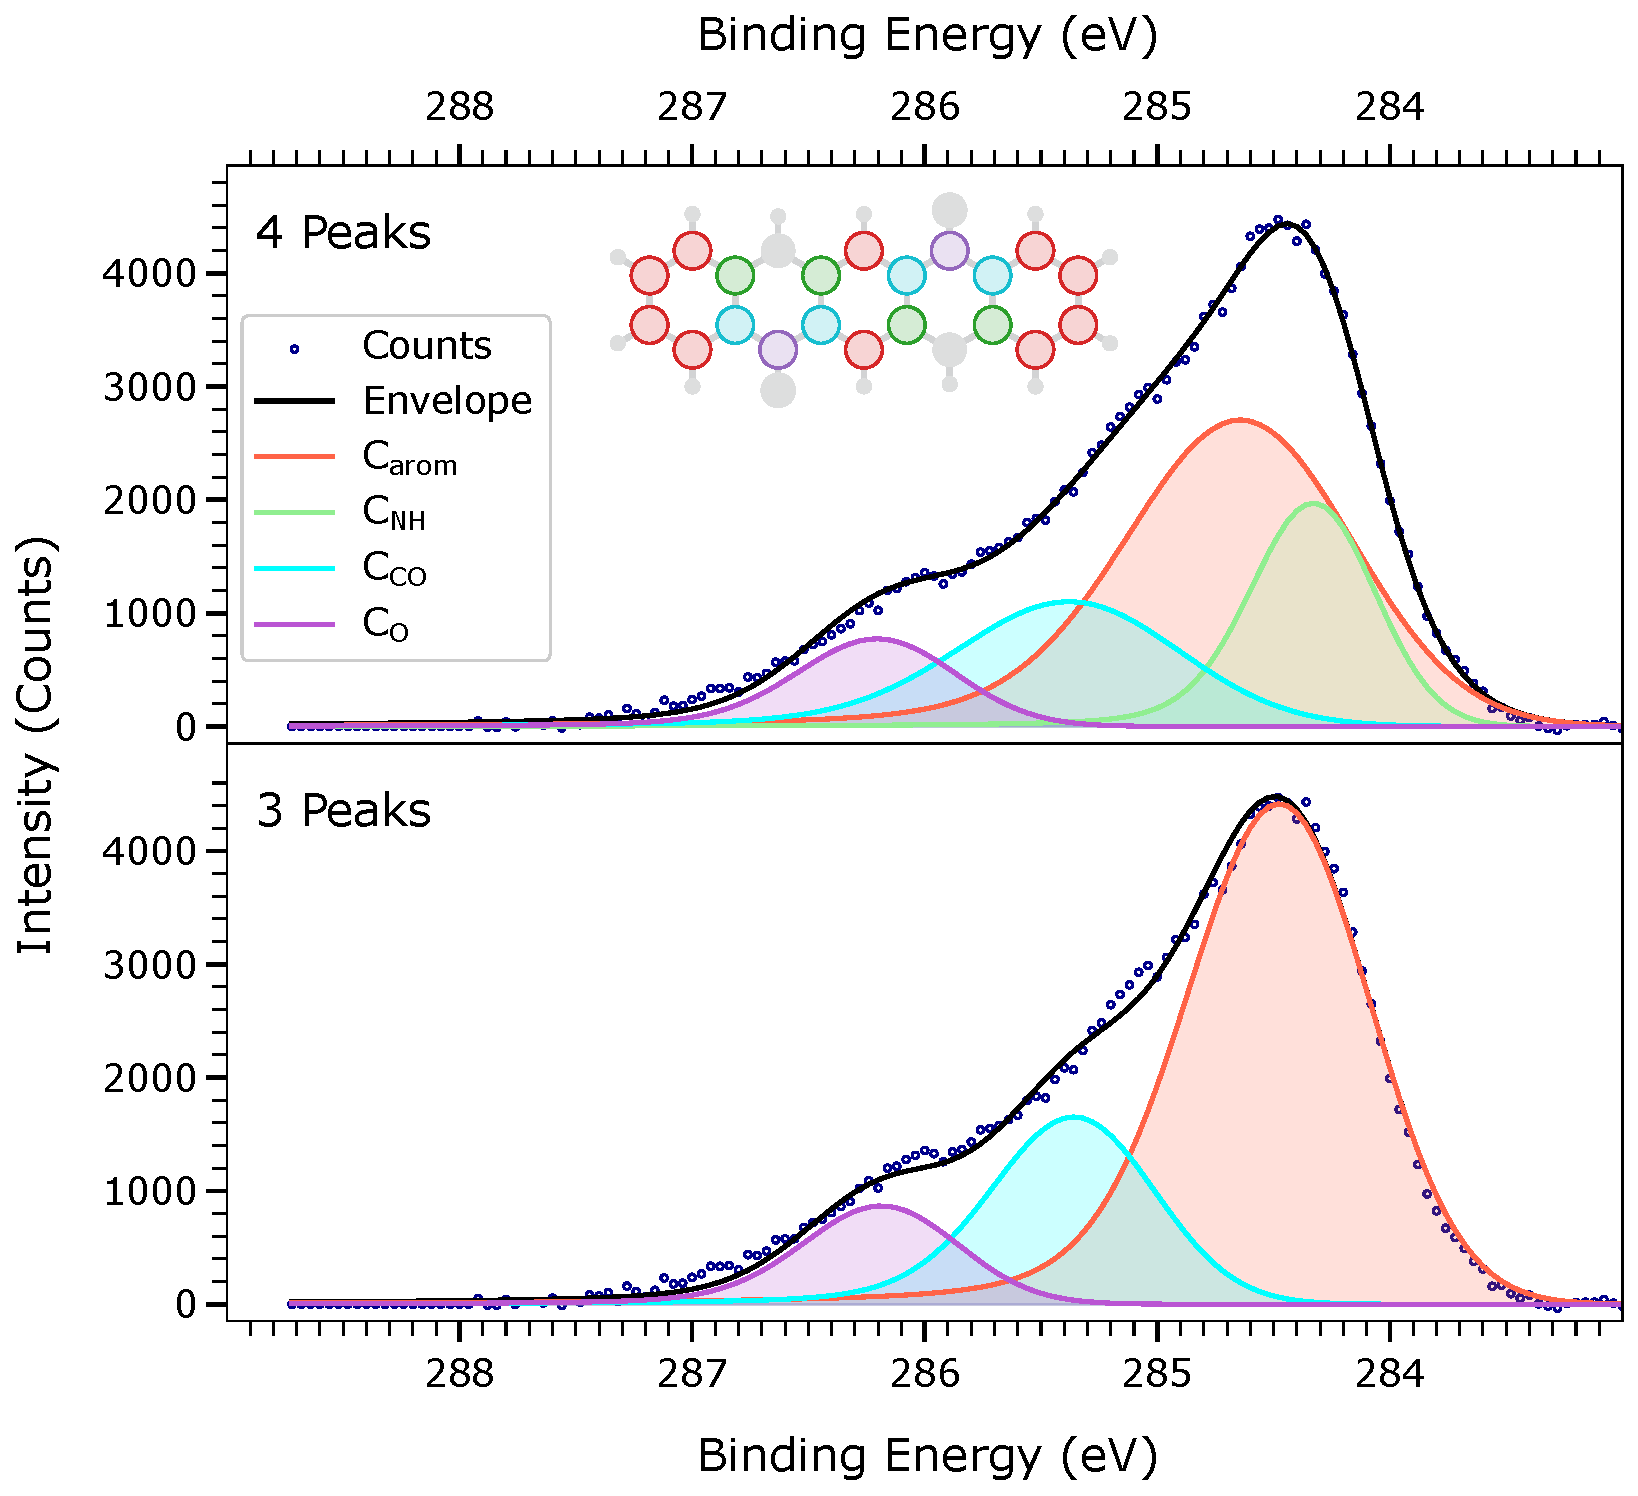
\includegraphics[width=0.7\textwidth]{images/XPS/C1s-FitModel-NIXSW.pdf}
\end{figure}

\end{frame}


\end{document}
